% !TeX root = ../main.tex
% Tám biểu đồ đã chèn; hai ảnh dashboard thật đang chờ bổ sung.
\chapter{Kết quả phân tích, kiểm thử và thảo luận}
\label{chap:ketqua}

\newcommand{\ghiChuHinh}[1]{\fbox{\parbox{0.92\linewidth}{\small\setstretch{1.1}\textbf{[CẦN CHÈN ẢNH]}\newline #1}}}

Nếu chỉ đếm số bản ghi, câu trả lời cho câu hỏi ``nhóm lỗi nào đáng chú ý nhất'' sẽ là \maCot{Other_Faults}, nhãn đông nhất nhưng cũng là nhãn gộp. Chương này cho thấy một câu trả lời khác. \maCot{K_Scatch} chỉ đứng thứ ba về số lượng, nhưng khi lần lượt đặt dòng thép, độ sáng, độ dày và diện tích vào cùng góc nhìn, đây là nhóm có hồ sơ rõ nét nhất trong dữ liệu, và vì thế là ứng viên cụ thể nhất cho việc kiểm chứng tiếp theo.

Câu chuyện đi theo thứ tự các câu hỏi. Q0 cho biết vì sao có thể tin các biểu đồ phía sau; Q1 xác định cơ cấu chung; Q2--Q5 tách dần từng chiều để làm hiện ra hồ sơ của \maCot{K_Scatch}; dashboard cho phép người đọc tự kiểm tra lại hồ sơ đó. Các phân tích dùng 1.941 bản ghi sau làm sạch, gồm 777 bản ghi A300 và 1.164 bản ghi A400. Đây đều là bản ghi lỗi, nên mọi tỷ trọng trong chương mô tả cơ cấu của tập lỗi, không phải tỷ lệ sản phẩm lỗi; giới hạn này và các giới hạn khác được tập hợp ở mục~\ref{sec:ch4thaoluan}.

\section{Vì sao có thể tin các biểu đồ: Q0}
\label{sec:ch4q0}

Biểu đồ cơ cấu chỉ có nghĩa khi mỗi thanh ứng với đúng một nhóm. Tệp thực hành ban đầu chưa đáp ứng điều đó: bảy nhãn được viết theo 28 cách, 70 ô đặc trưng bị thiếu, 20 dòng trùng, và một số chỉ số mang giá trị không thể là thật, như \maCot{Empty_Index} bằng 2031 trong khi giá trị tính từ diện tích và khung bao chỉ xấp xỉ 0,2031. Bảng~\ref{tab:ch4chatluong} tóm tắt trạng thái dữ liệu trước và sau quy trình đã trình bày ở Chương~3.

\begin{center}\begin{minipage}{\linewidth}
\captionof{table}{Kết quả Q0 theo từng trạng thái dữ liệu}
\label{tab:ch4chatluong}
\small\setstretch{1.1}
\begin{tabularx}{\linewidth}{@{}Y p{3.1cm}p{3.1cm}@{}}
\toprule
Nội dung kiểm tra & Trước xử lý & Kết quả xử lý \\
\midrule
Số bản ghi & 1.961 & 1.941; loại 20 dòng trùng \\
Biểu diễn nhãn & 28 cách viết & 7 nhãn chuẩn \\
Ô thiếu trong 27 đặc trưng & 70 ô ở bảng đầu vào & Còn 67 sau loại trùng; khôi phục đủ \\
Ô sai lệch do kiểm tra nội tại bổ sung & 16 ô được gắn cờ trước khôi phục & 16 ô có giá trị sửa đối chiếu UCI \\
Ngày trong hồ sơ thực hành & 27 biểu diễn & 5 ngày mô phỏng; giữ ngày gốc \\
Khóa ghép tọa độ & Kiểm tra ở cả hai nguồn & Ghép một--một, không tăng số dòng \\
Đặc trưng sau khôi phục & 27 đặc trưng mỗi bản ghi & 52.407 ô khớp nguồn tham chiếu \\
\bottomrule
\end{tabularx}
\end{minipage}\end{center}

Hai kết quả trong bảng có vai trò khác nhau. Lượt rà soát nội tại phát hiện 16 ô sai lệch (mười ô \maCot{Empty_Index}, sáu ô \maCot{Log_Y_Index}) chỉ từ quan hệ giữa các cột trên cùng dòng, trước khi dùng đến UCI. Còn việc toàn bộ $1.941\times27=52.407$ ô khớp UCI chỉ xác nhận phép ghép và khôi phục đã làm đúng, vì chính UCI cung cấp giá trị điền và sửa.

Một quyết định ở bước này sẽ quay lại ở cuối câu chuyện: 395 bản ghi có diện tích vượt hàng rào IQR toàn tập được \emph{giữ lại}, vì giá trị của chúng khớp nguồn. Mục~\ref{sec:ch4q5} sẽ cho thấy nếu xóa chúng thì bức tranh cơ cấu thay đổi ra sao.

\section{Ba nhãn chiếm ba phần tư số bản ghi: Q1}
\label{sec:ch4q1}

Bức tranh đầu tiên là mức tập trung về số lượng. Ba nhãn \maCot{Other_Faults}, \maCot{Bumps} và \maCot{K_Scatch} chứa 1.466 trong 1.941 bản ghi, tương ứng 75,53\%. Đường lũy kế trên Hình~\ref{fig:ch4pareto} cho thấy phải thêm nhãn thứ tư, \maCot{Z_Scratch}, thì tỷ trọng mới vượt 80\%.

\begin{center}\begin{minipage}{\linewidth}
\centering
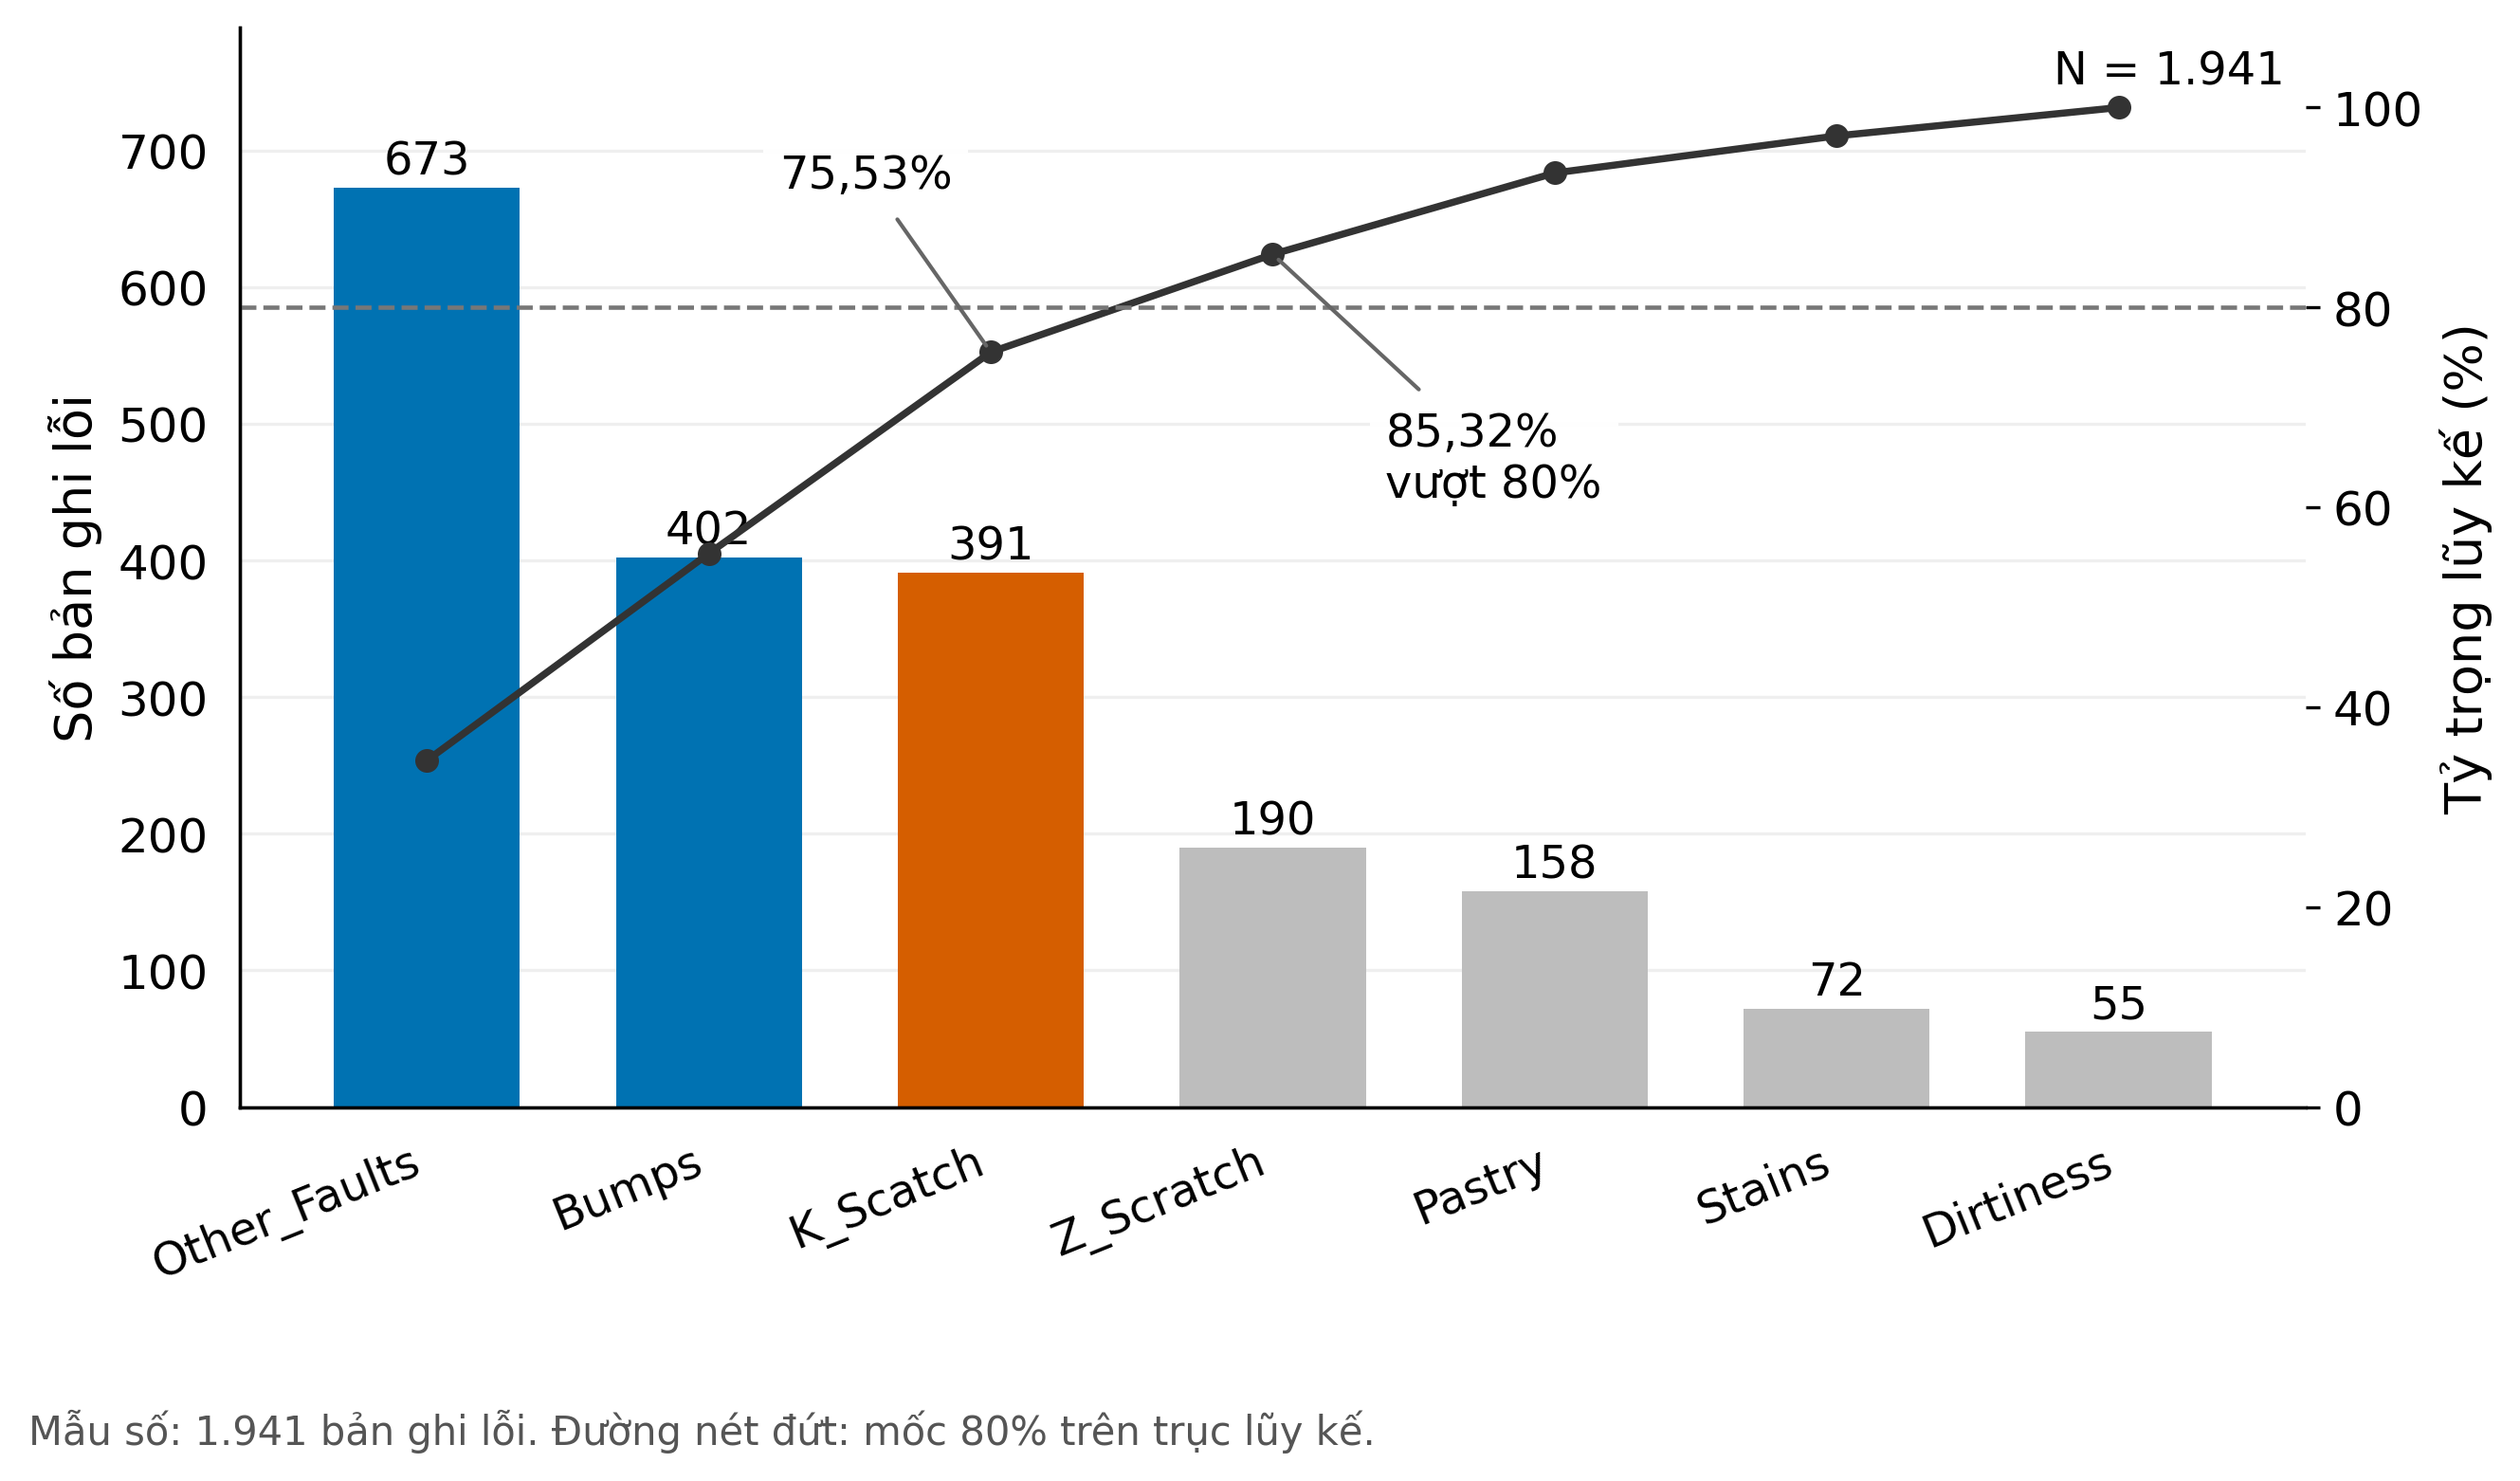
\includegraphics[width=\linewidth]{figures/chuong4/ch4_01_pareto.png}
\captionof{figure}{Ba nhãn đầu chiếm 75,53\% số bản ghi; cần bốn nhãn để vượt 80\%}
\label{fig:ch4pareto}
\end{minipage}\end{center}

\begin{center}\begin{minipage}{\linewidth}
\captionof{table}{Số lượng, tỷ trọng và tỷ trọng lũy kế theo nhãn}
\label{tab:ch4cocau}
\small\setstretch{1.1}
\begin{tabularx}{\linewidth}{@{}Y rrr@{}}
\toprule
Nhãn & Số bản ghi & Tỷ trọng (\%) & Lũy kế (\%) \\
\midrule
\maCot{Other_Faults} & 673 & 34,67 & 34,67 \\
\maCot{Bumps} & 402 & 20,71 & 55,38 \\
\maCot{K_Scatch} & 391 & 20,14 & 75,53 \\
\maCot{Z_Scratch} & 190 & 9,79 & 85,32 \\
\maCot{Pastry} & 158 & 8,14 & 93,46 \\
\maCot{Stains} & 72 & 3,71 & 97,17 \\
\maCot{Dirtiness} & 55 & 2,83 & 100,00 \\
\midrule
Tổng & 1.941 & 100,00 & \\
\bottomrule
\end{tabularx}
\end{minipage}\end{center}

Nhãn đông nhất, \maCot{Other_Faults} với 673 bản ghi, lại là nhãn ít nói lên điều gì nhất: đây là nhóm gộp, và dữ liệu không cho biết 673 bản ghi này thuộc một hay nhiều loại lỗi. Điều đáng chú ý hơn nằm ở hai thanh tiếp theo. \maCot{Bumps} có 402 bản ghi, \maCot{K_Scatch} có 391, chỉ chênh nhau 11. Theo số đếm, hai nhóm gần như ngang nhau. Các mục sau sẽ cho thấy chúng khác nhau đến mức nào.

Bảng~\ref{tab:ch4cocau} cũng nhắc một điều cần mang theo khi đọc các hình phía sau: nhóm lớn nhất gấp nhóm nhỏ nhất khoảng 12,24 lần. Trên scatter, nhóm đông tự nhiên tạo vùng điểm dày hơn; trên boxplot, nhóm ít quan sát cần được đọc cùng cỡ mẫu.

\section{Hai nhãn ngang nhau, hai dòng thép khác nhau: Q2}
\label{sec:ch4q2}

Khi tách theo dòng thép, sự ngang nhau giữa \maCot{Bumps} và \maCot{K_Scatch} biến mất. Trên Hình~\ref{fig:ch4thepsoluong}, \maCot{Bumps} trải trên cả hai dòng, với 279 bản ghi A300 và 123 bản ghi A400. \maCot{K_Scatch} thì gần như chỉ có ở A400: 390 bản ghi, so với đúng một bản ghi trên A300.

\begin{center}\begin{minipage}{\linewidth}
\centering
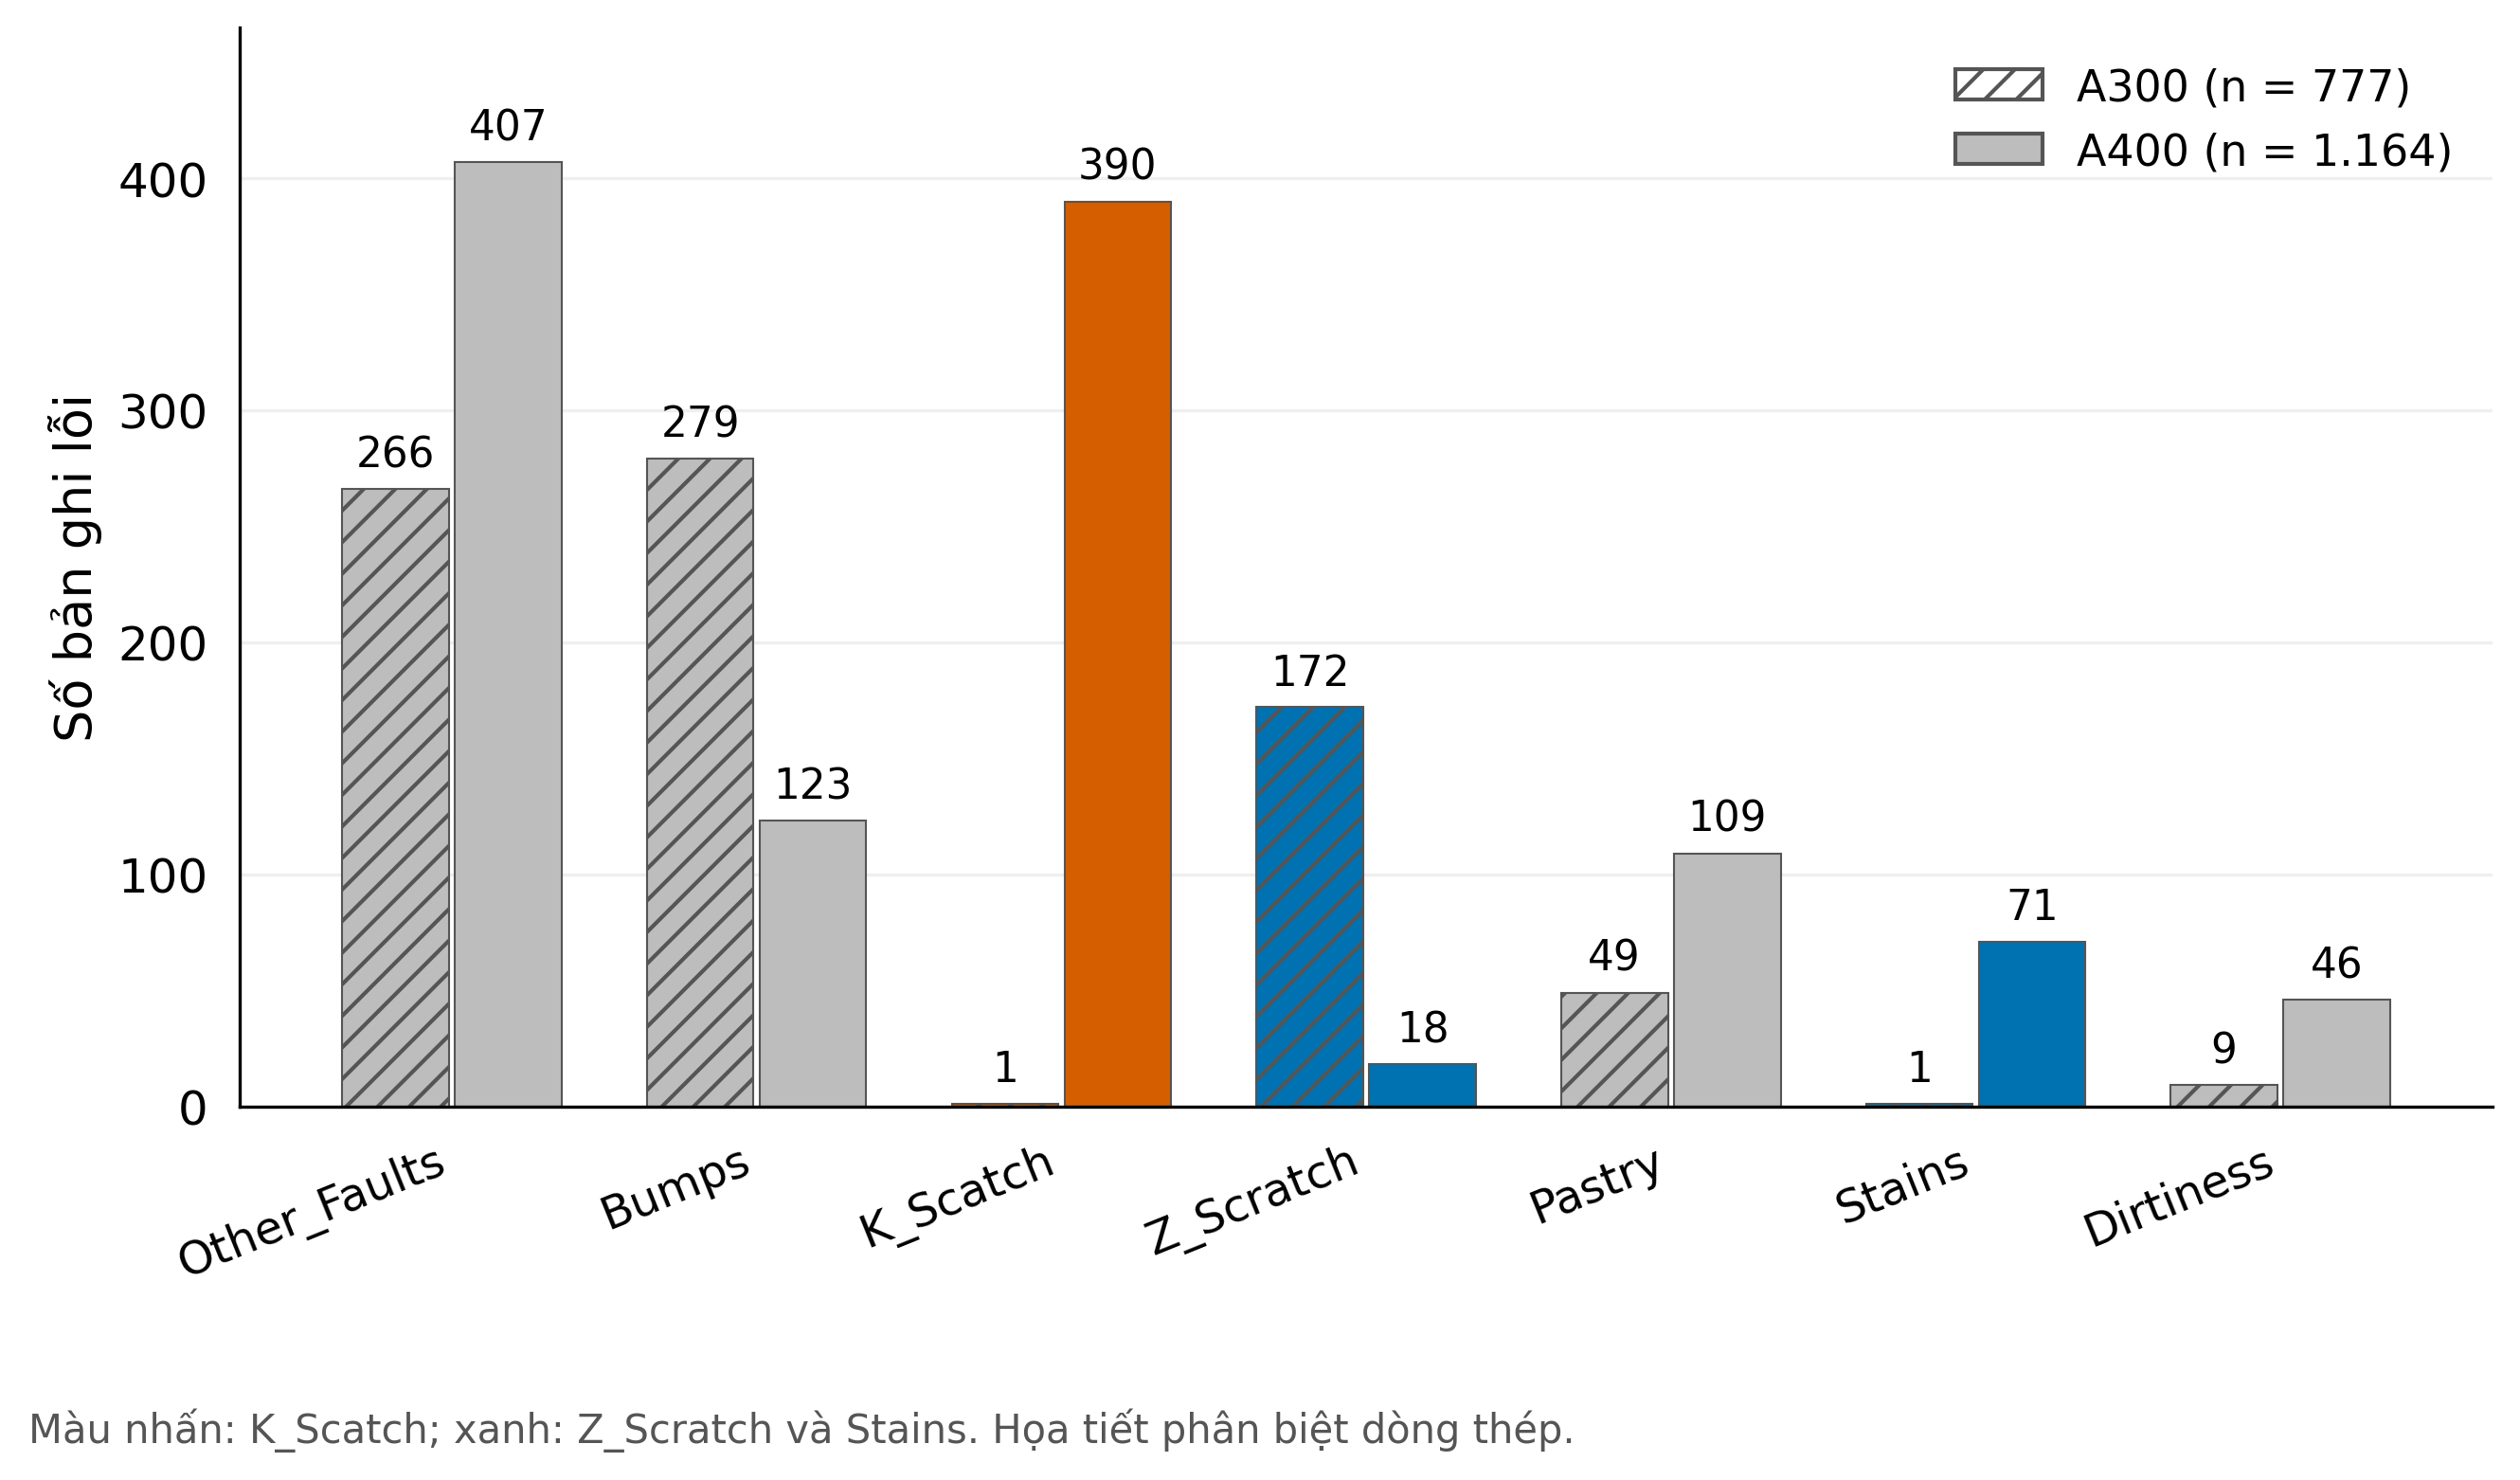
\includegraphics[width=\linewidth]{figures/chuong4/ch4_02_thep_so_luong.png}
\captionof{figure}{K\_Scatch gần như chỉ xuất hiện trên A400}
\label{fig:ch4thepsoluong}
\end{minipage}\end{center}

Vì hai dòng thép có cỡ mẫu khác nhau (777 và 1.164), so sánh số đếm chưa đủ. Hình~\ref{fig:ch4theptytrong} đưa mỗi dòng về một cột 100\% để thấy cơ cấu bên trong. Ở A300, \maCot{Bumps} chiếm 35,91\% và \maCot{Z_Scratch} chiếm 22,14\%. Ở A400, \maCot{K_Scatch} chiếm 33,51\%, còn \maCot{Bumps} chỉ còn 10,57\%. Phần \maCot{Other_Faults} gần như không đổi giữa hai dòng, 34,23\% và 34,97\%; khác biệt nằm ở các nhãn cụ thể.

\begin{center}\begin{minipage}{\linewidth}
\centering
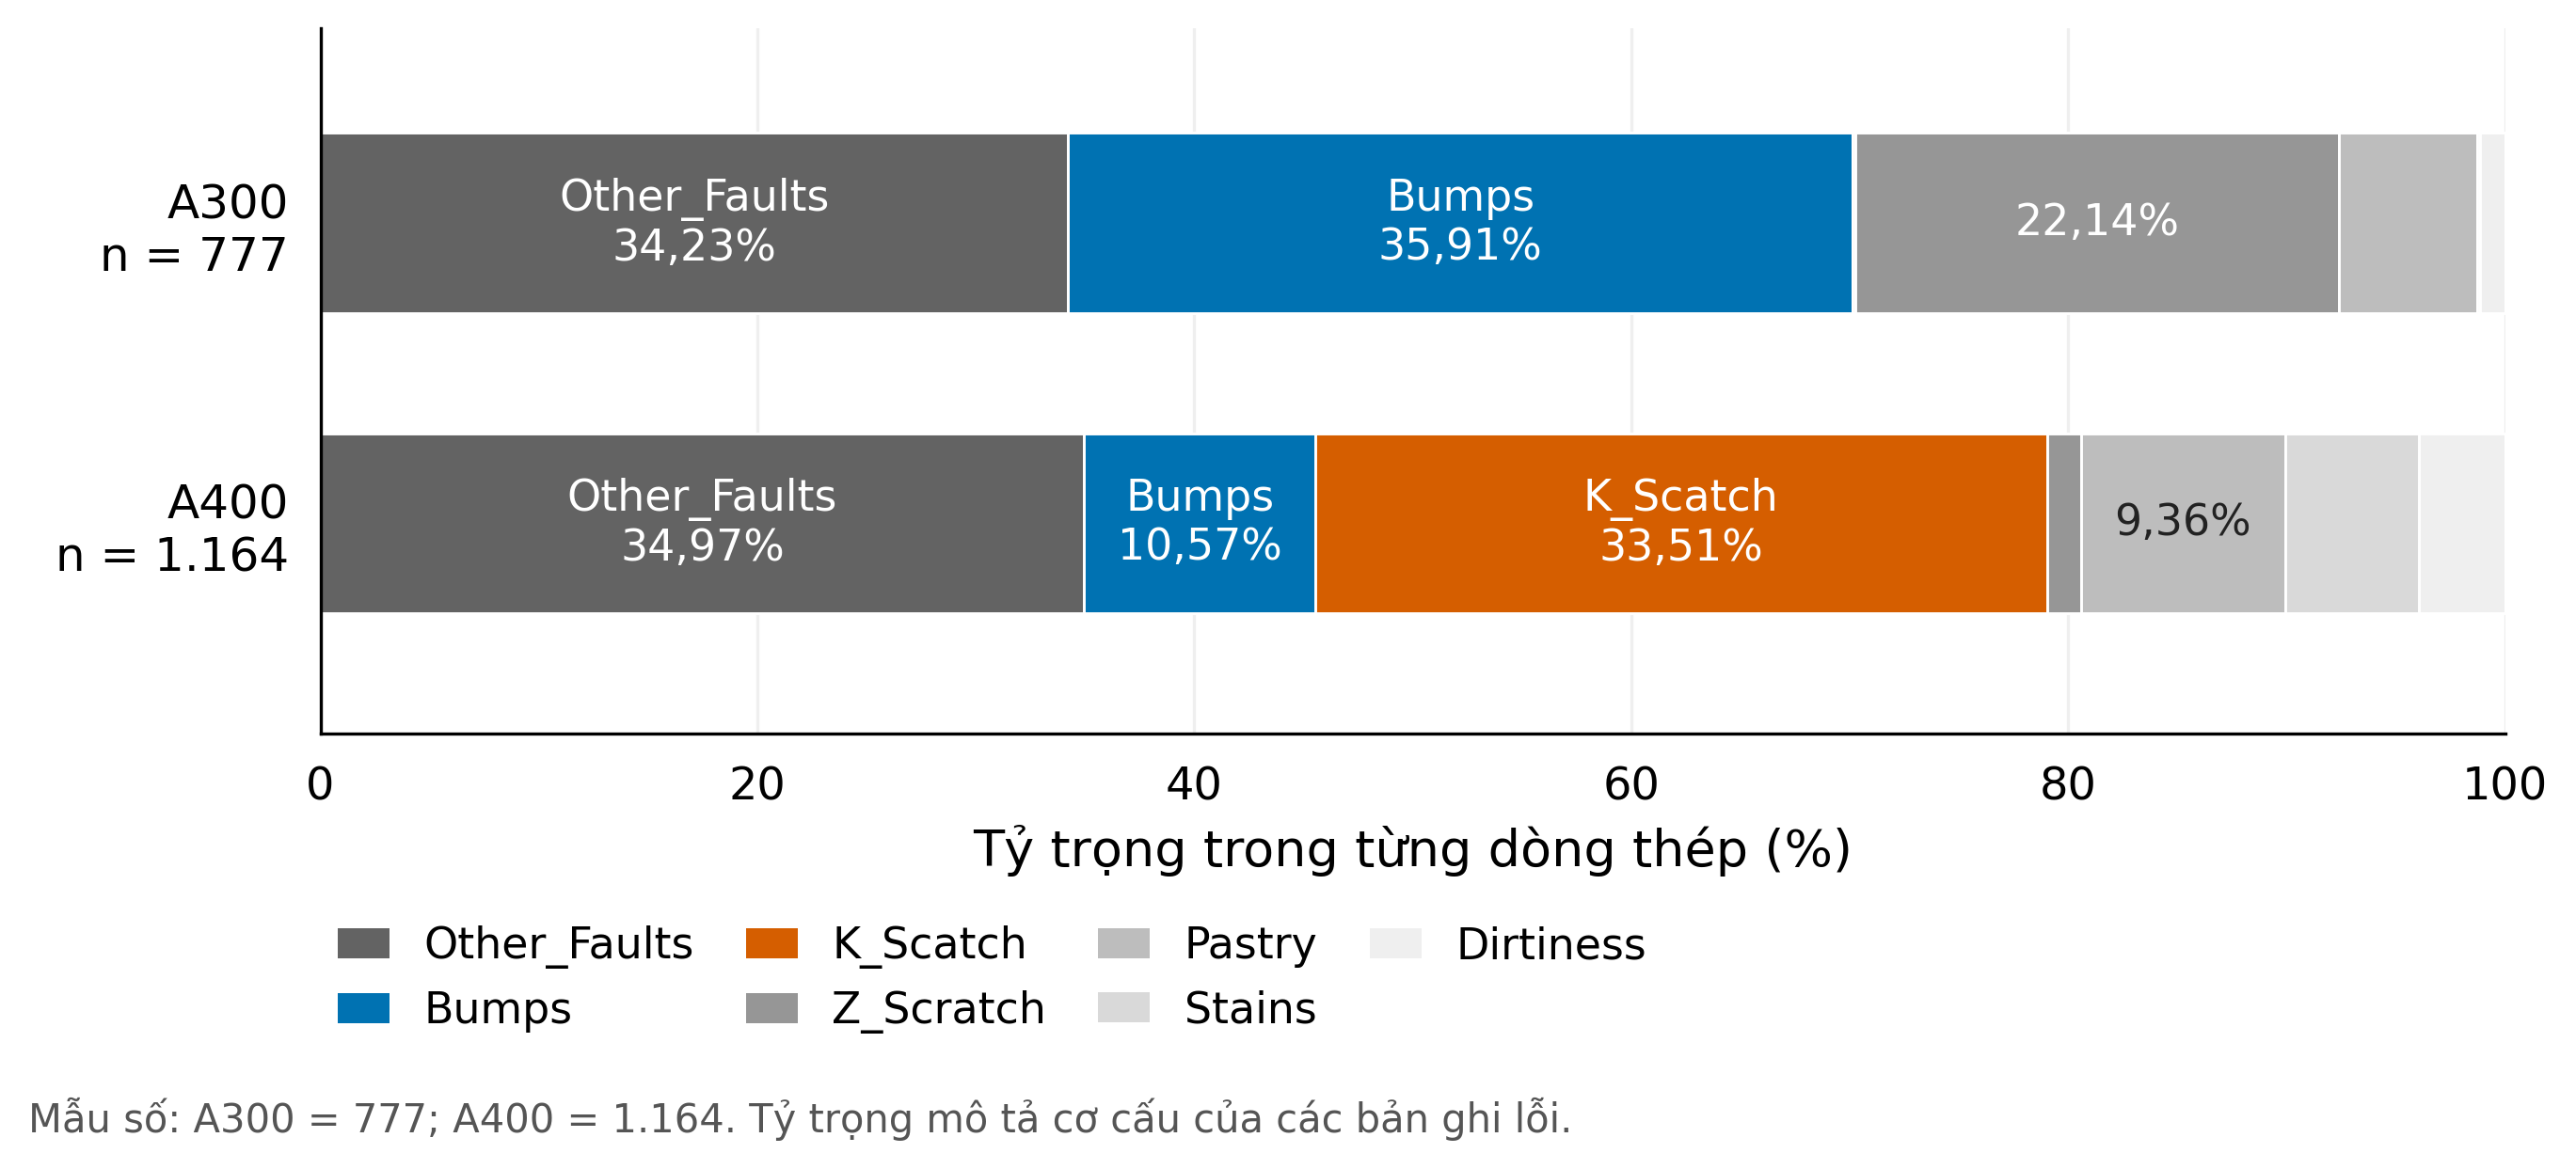
\includegraphics[width=\linewidth]{figures/chuong4/ch4_03_thep_ty_trong.png}
\captionof{figure}{Trong cơ cấu lỗi, A300 nổi bật Bumps, A400 nổi bật K\_Scatch}
\label{fig:ch4theptytrong}
\end{minipage}\end{center}

Câu hỏi Q2 lại hỏi theo chiều ngược: trong mỗi nhãn, bao nhiêu phần trăm bản ghi nằm trên cùng một dòng thép? Đổi mẫu số sang tổng của từng nhãn, Bảng~\ref{tab:ch4taptrung} cho thấy ba nhãn vượt mốc 90\% ở công thức~\ref{eq:tieuchiq2}: \maCot{K_Scatch} (99,74\% ở A400), \maCot{Stains} (98,61\% ở A400) và \maCot{Z_Scratch} (90,53\% ở A300).

\begin{center}\begin{minipage}{\linewidth}
\captionof{table}{Phân bố A300/A400 trong từng nhãn và mốc tập trung trên 90\%}
\label{tab:ch4taptrung}
\small\setstretch{1.1}
\begin{tabularx}{\linewidth}{@{}Y rr p{2.0cm}r@{}}
\toprule
Nhãn & A300 & A400 & Dòng tập trung & Tỷ trọng trong nhãn (\%) \\
\midrule
\maCot{Other_Faults} & 266 & 407 & A400 & 60,48 \\
\maCot{Bumps} & 279 & 123 & A300 & 69,40 \\
\maCot{K_Scatch} & 1 & 390 & A400 & \textbf{99,74} \\
\maCot{Z_Scratch} & 172 & 18 & A300 & \textbf{90,53} \\
\maCot{Pastry} & 49 & 109 & A400 & 68,99 \\
\maCot{Stains} & 1 & 71 & A400 & \textbf{98,61} \\
\maCot{Dirtiness} & 9 & 46 & A400 & 83,64 \\
\bottomrule
\end{tabularx}
\end{minipage}\end{center}

Với \maCot{K_Scatch}, hai mẫu số cho hai câu trả lời khác hẳn nhau từ cùng một tử số:
\begin{equation}
\frac{390}{391}\times100\%\approx99{,}74\%,
\qquad
\frac{390}{1.164}\times100\%\approx33{,}51\%.
\label{eq:ch4mauso}
\end{equation}
Con số thứ nhất nói \maCot{K_Scatch} tập trung ở đâu; con số thứ hai nói nhãn này chiếm bao nhiêu trong lỗi của A400. Đọc nhầm hai con số này là cách nhanh nhất để biến một mô tả về bản ghi lỗi thành một khẳng định sai về chất lượng sản phẩm A400.

Sau Q2, \maCot{K_Scatch} không còn chỉ là ``nhãn thứ ba''. Đó là nhóm gần như nằm trọn trong A400. Câu hỏi tiếp theo là nhóm này có khác biệt ở chính đặc trưng của bản ghi hay không.

\section{Độ sáng tách được phần trung tâm của K\_Scatch: Q3}
\label{sec:ch4q3}

Hình~\ref{fig:ch4scatter} đặt mỗi bản ghi theo độ sáng tối thiểu và tối đa. Khi các nhãn khác được làm xám, \maCot{K_Scatch} hiện ra thành những dải ngang ở phía độ sáng tối thiểu thấp, chủ yếu trong khoảng 20--50. Nhưng hình cũng cho thấy một nhánh \maCot{K_Scatch} chạy dọc đường chéo phía trên, tới độ sáng tối thiểu gần 200. Hệ số Pearson toàn tập là 0,4296, một liên hệ tuyến tính dương ở mức vừa.

\begin{center}\begin{minipage}{\linewidth}
\centering
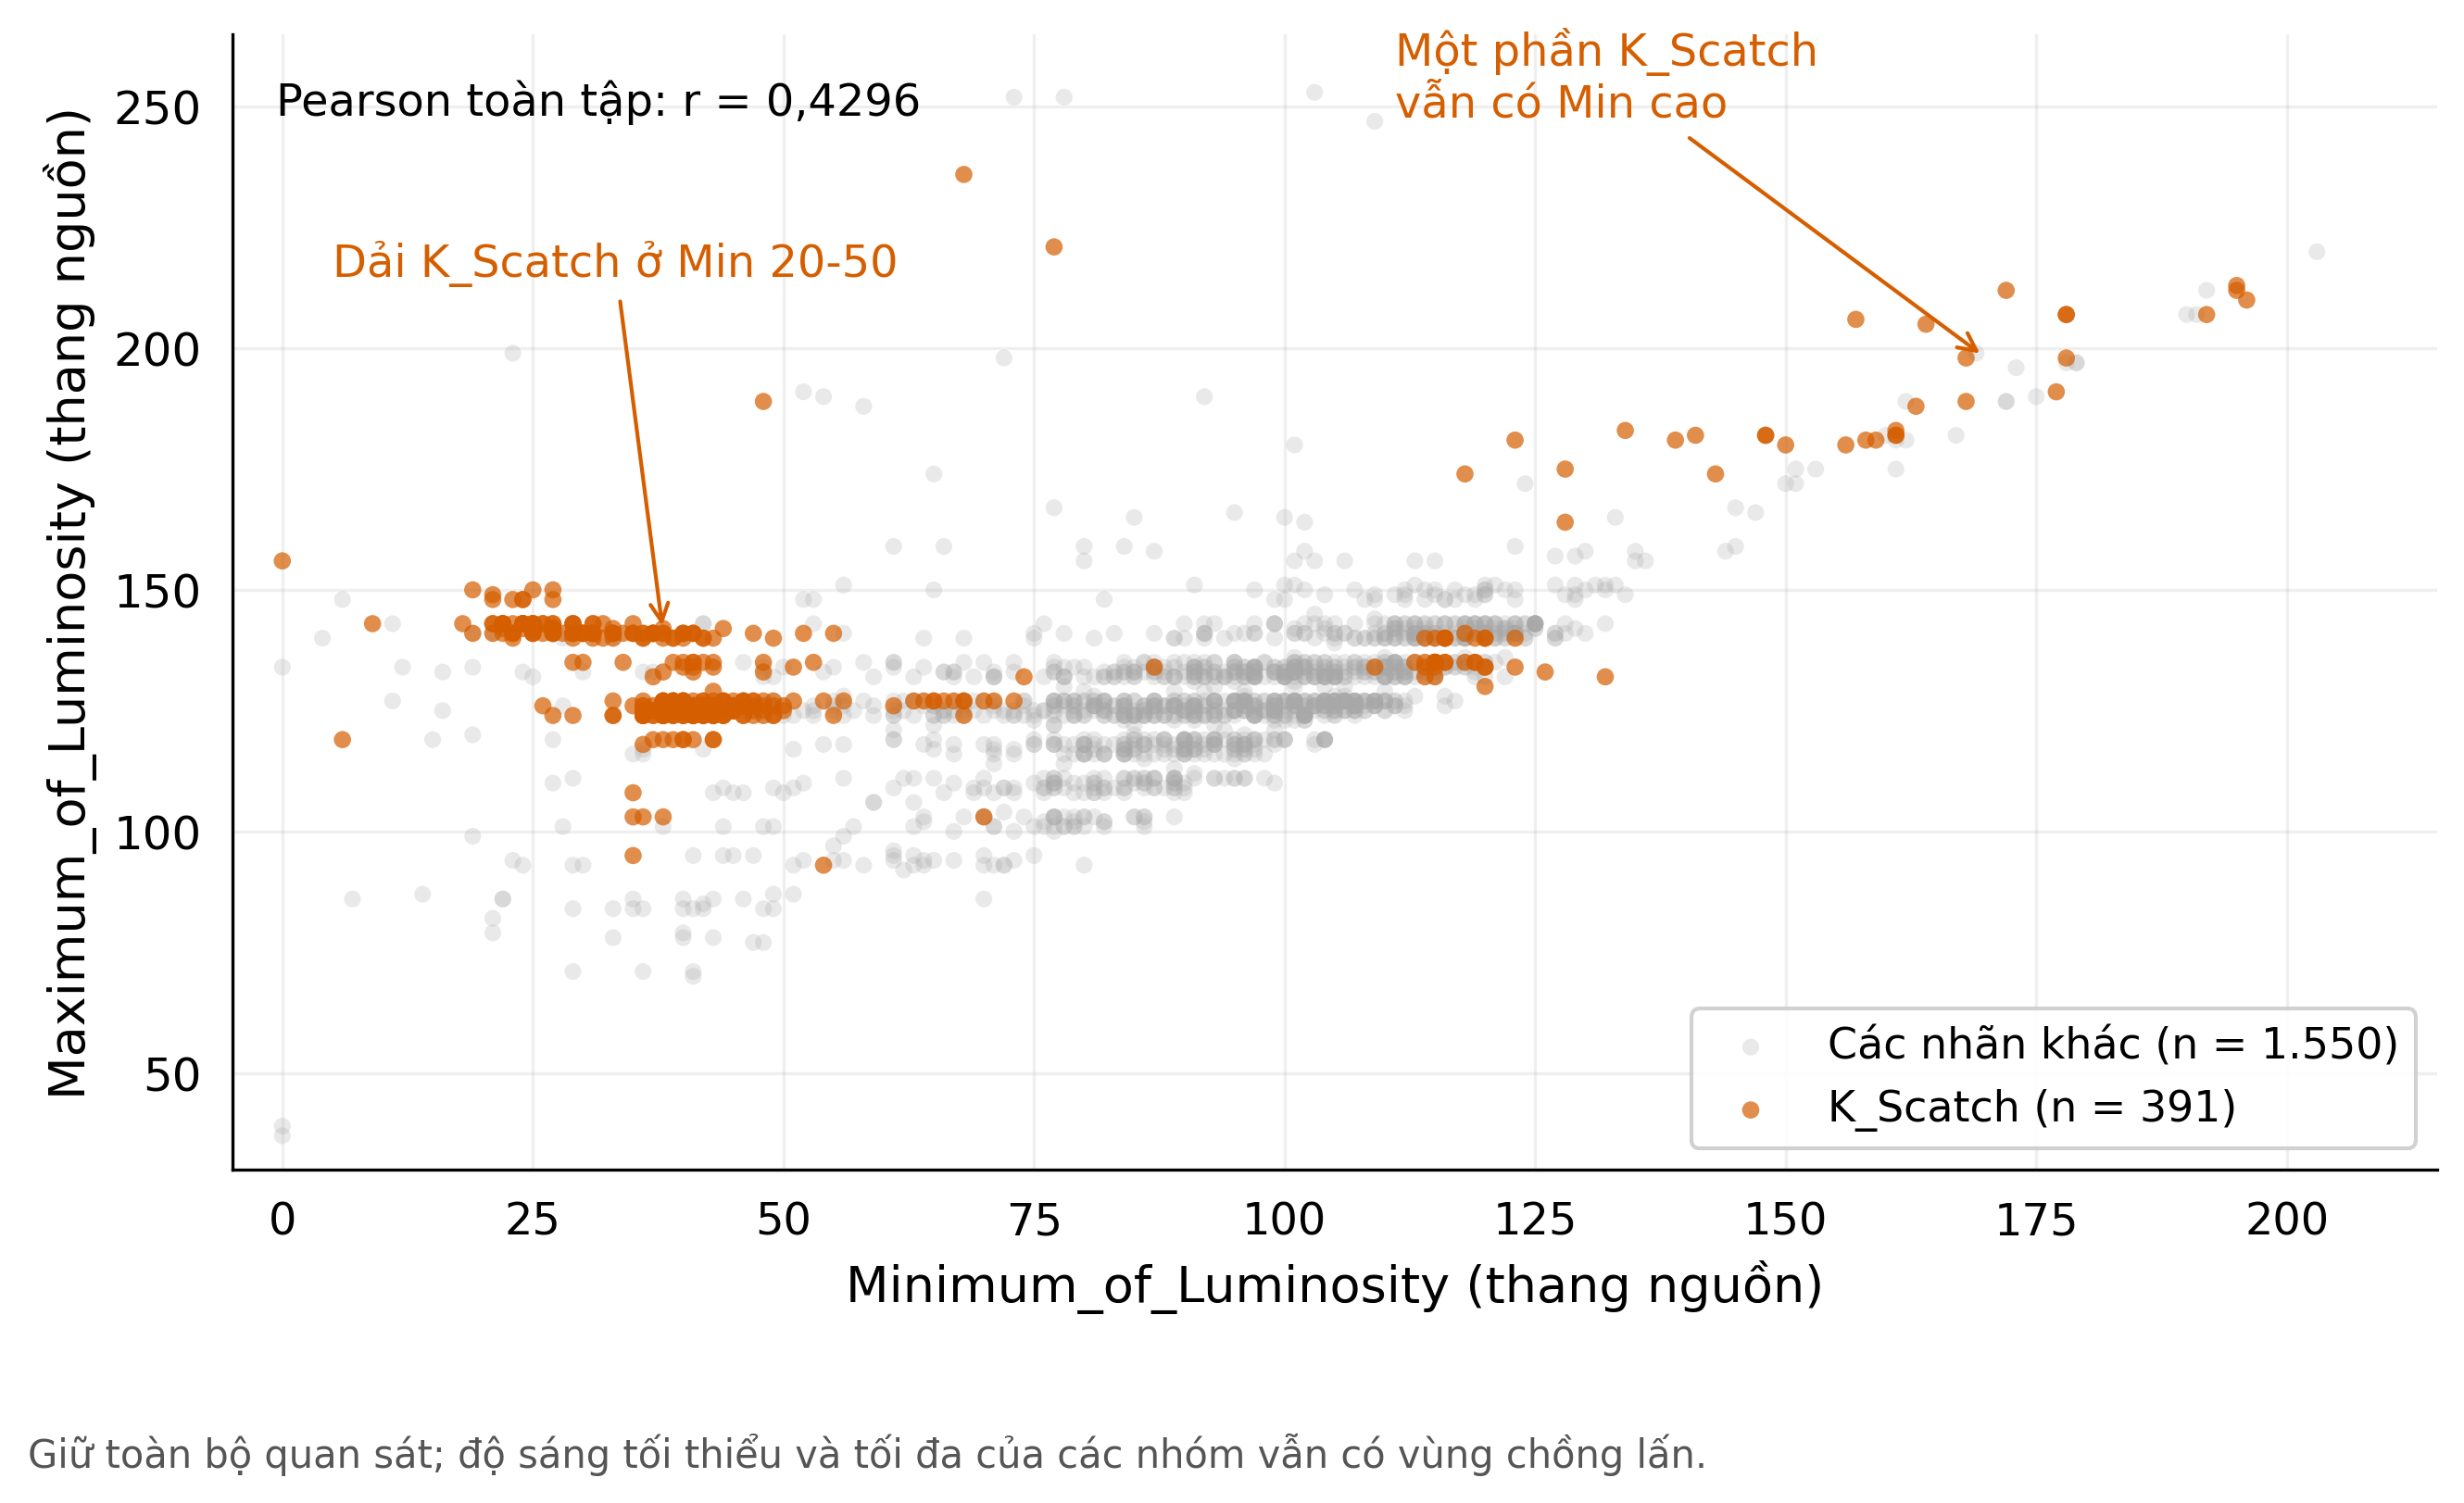
\includegraphics[width=\linewidth]{figures/chuong4/ch4_04_scatter_do_sang.png}
\captionof{figure}{K\_Scatch dồn về phía độ sáng tối thiểu thấp, nhưng không tách hoàn toàn}
\label{fig:ch4scatter}
\end{minipage}\end{center}

Scatter có nhiều điểm chồng nhau nên khó so sánh chính xác. Hình~\ref{fig:ch4iqrsang} thu gọn mỗi nhãn về trung vị và khoảng P25--P75 của độ sáng tối thiểu. Ở góc nhìn này, khoảng 35--49 của \maCot{K_Scatch} đứng tách hẳn khỏi sáu nhãn còn lại. Khoảng gần nhất là của \maCot{Pastry}, bắt đầu từ 64, cách 15 đơn vị thang nguồn. \maCot{K_Scatch} là nhãn duy nhất đáp ứng tiêu chí không chồng IQR ở công thức~\ref{eq:tieuchiq3}.

\begin{center}\begin{minipage}{\linewidth}
\centering
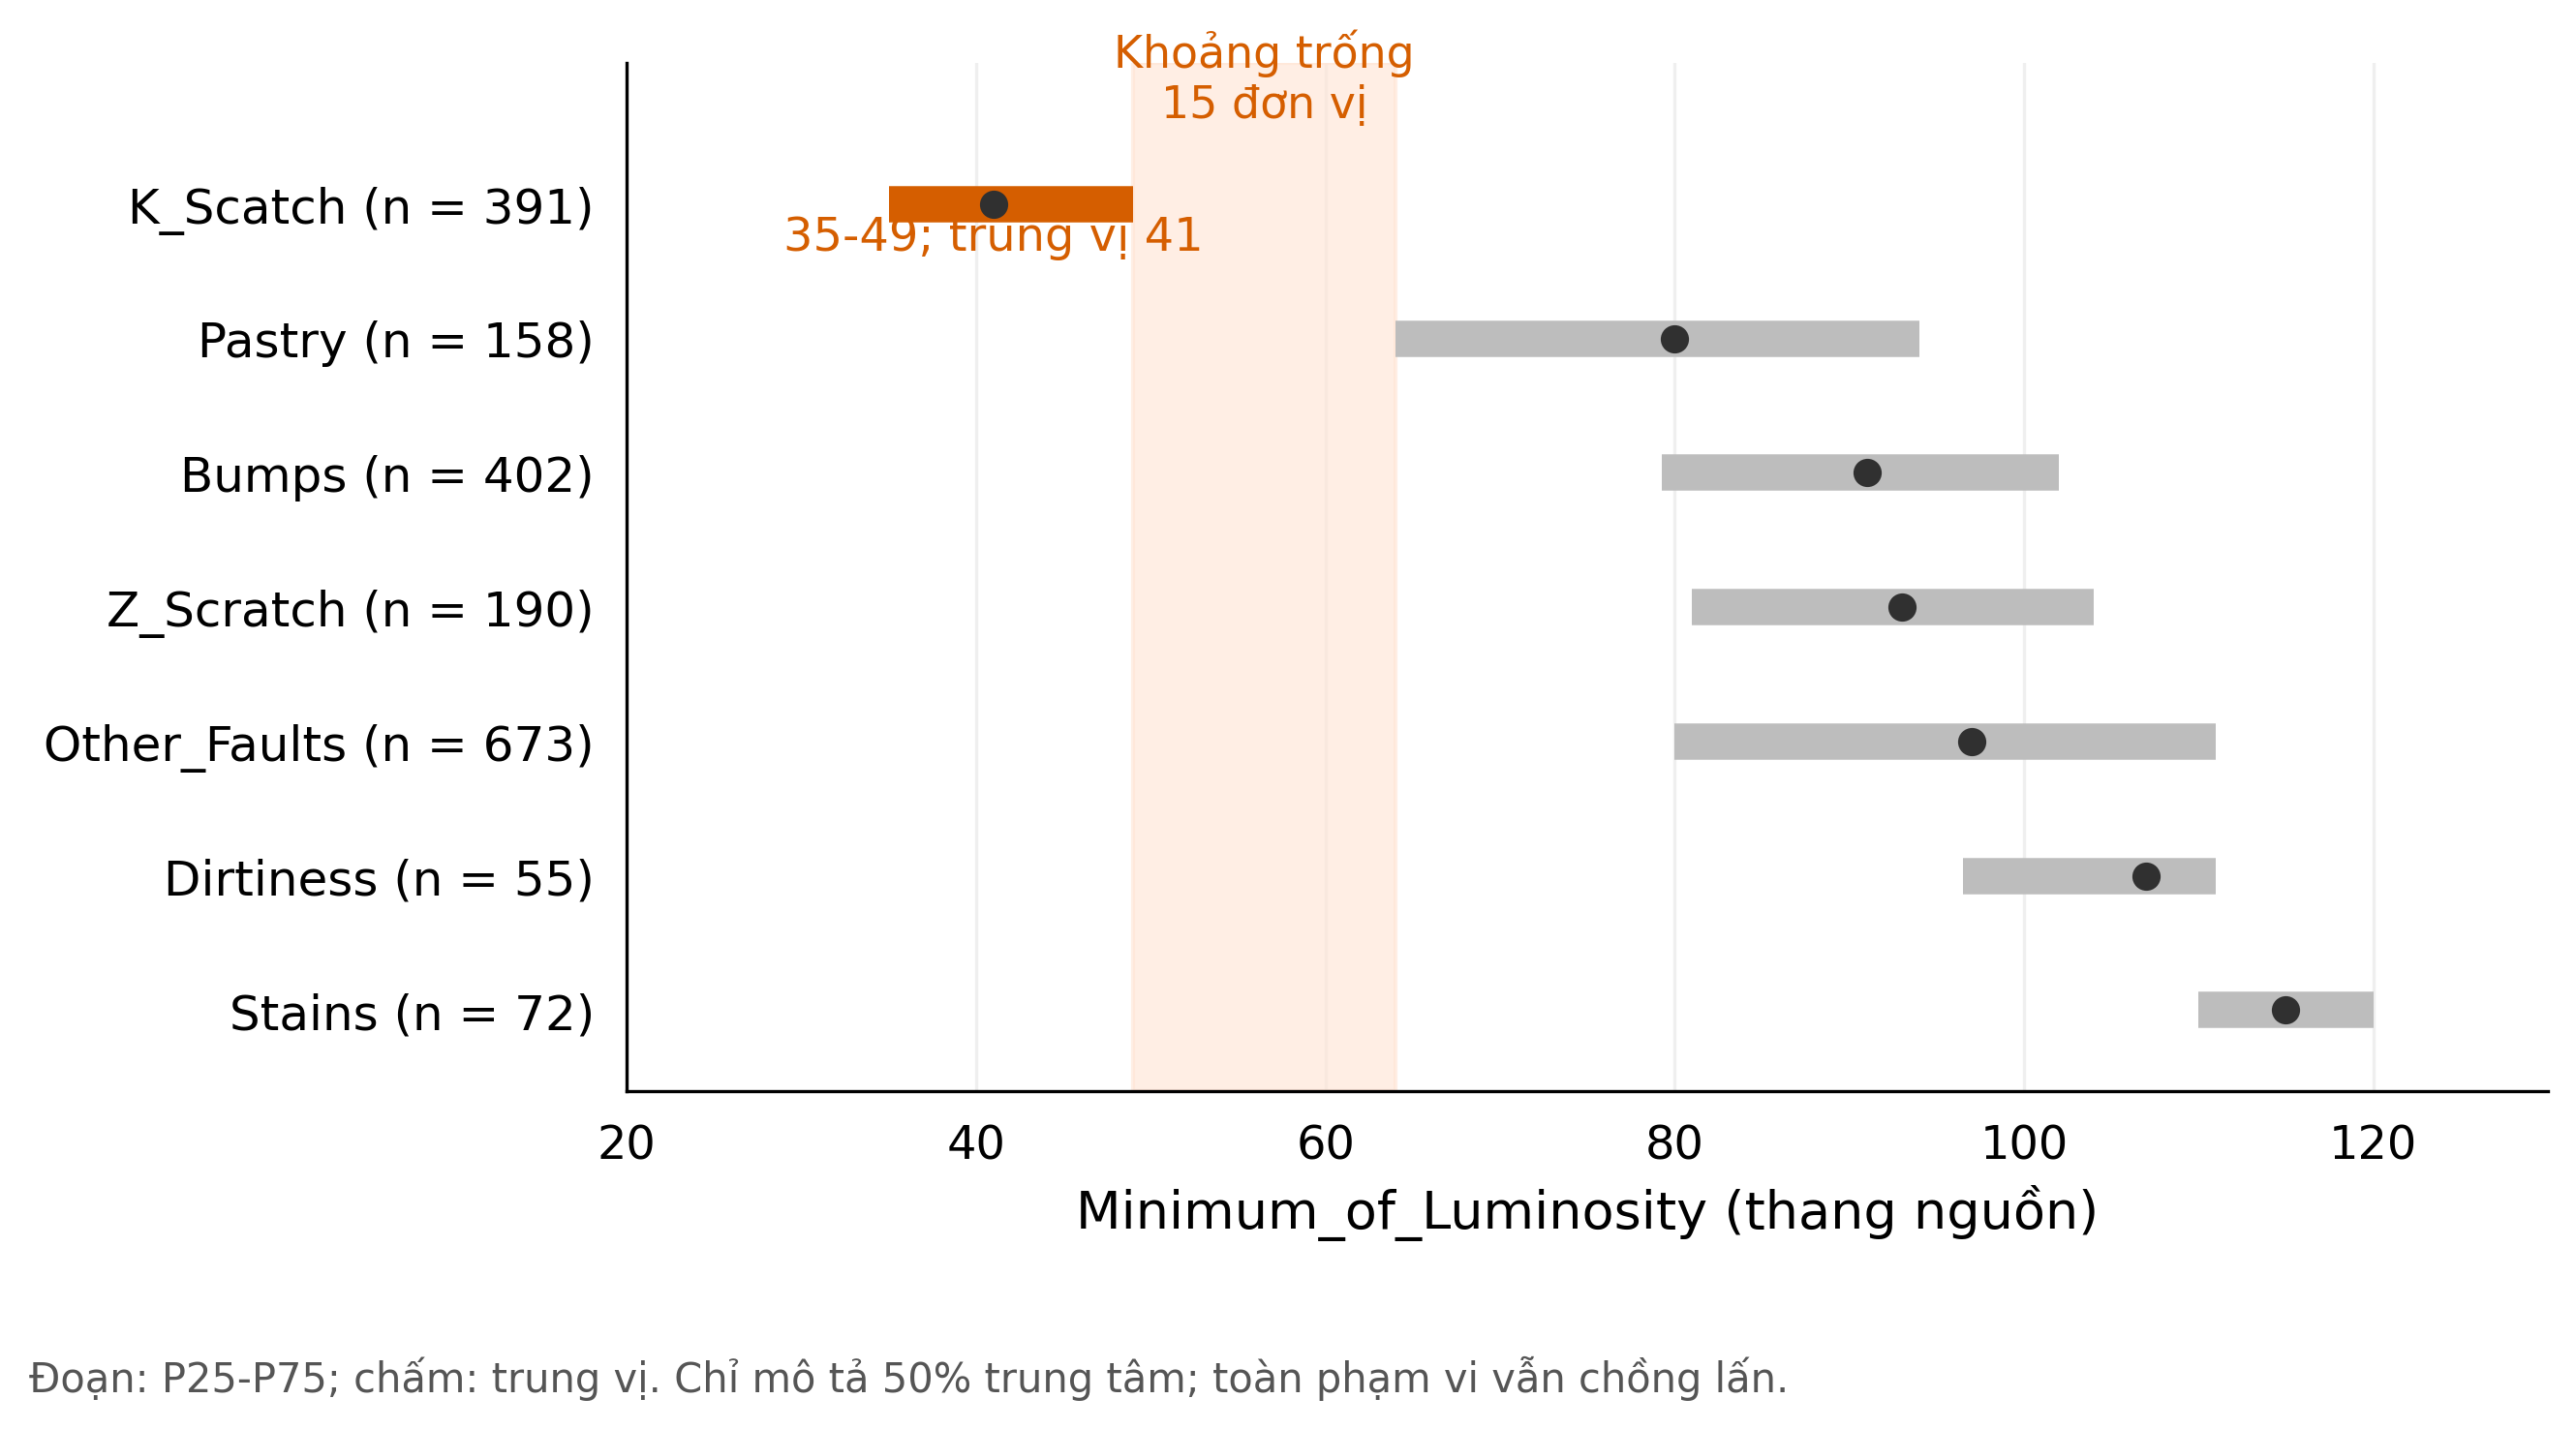
\includegraphics[width=\linewidth]{figures/chuong4/ch4_05_iqr_do_sang.png}
\captionof{figure}{Phần trung tâm độ sáng tối thiểu của K\_Scatch không chồng với nhãn nào khác}
\label{fig:ch4iqrsang}
\end{minipage}\end{center}

\begin{center}\begin{minipage}{\linewidth}
\captionof{table}{Phần trung tâm phân bố độ sáng tối thiểu và tối đa}
\label{tab:ch4dosang}
\small\setstretch{1.1}
\begin{tabularx}{\linewidth}{@{}Y r r p{2.1cm}r p{2.1cm}@{}}
\toprule
Nhãn & $N$ & Trung vị Min & P25--P75 Min & Trung vị Max & P25--P75 Max \\
\midrule
\maCot{Other_Faults} & 673 & 97 & 80--111 & 127 & 119--140 \\
\maCot{Bumps} & 402 & 91 & 79,25--102 & 127 & 124--134 \\
\maCot{K_Scatch} & 391 & 41 & \textbf{35--49} & 134 & 126--141 \\
\maCot{Z_Scratch} & 190 & 93 & 81--104 & 124 & 111--132 \\
\maCot{Pastry} & 158 & 80 & 64--94 & 126 & 119--133 \\
\maCot{Stains} & 72 & 115 & 110--120 & 140 & 135--142 \\
\maCot{Dirtiness} & 55 & 107 & 96,5--111 & 132 & 127--140 \\
\bottomrule
\end{tabularx}
\end{minipage}\end{center}

Hai hình cần được đọc cùng nhau. Hình~\ref{fig:ch4iqrsang} cho thấy phần trung tâm của \maCot{K_Scatch} khác biệt; Hình~\ref{fig:ch4scatter} nhắc rằng toàn bộ phạm vi độ sáng tối thiểu của nhóm, từ 0 đến 196, vẫn chồng với các nhãn khác. Ở độ sáng tối đa, IQR 126--141 của \maCot{K_Scatch} cũng chồng với nhiều nhóm. Đây là một dấu hiệu ở phần trung tâm, không phải một ngưỡng để gán nhãn cho bản ghi mới. Thêm vào đó, tiêu chí này được đặt ra sau khi đã quan sát dữ liệu.

Hồ sơ của \maCot{K_Scatch} giờ có thêm một nét: nằm trên A400 và có độ sáng tối thiểu thấp ở phần trung tâm. Mục tiếp theo xem độ dày.

\section{Độ dày: một giá trị cho K\_Scatch, nhiều giá trị cho nhóm khác: Q4}
\label{sec:ch4q4}

Trên toàn tập, độ dày dao động rộng, với 76,30\% bản ghi nằm trong khoảng 40--80 và trung vị 70. Khi chia theo nhãn, Bảng~\ref{tab:ch4doday} cho thấy các nhóm khác nhau rõ về độ rộng phân bố. \maCot{Other_Faults} và \maCot{Bumps} có cùng trung vị 70, nhưng IQR lần lượt là 90 và 20. Ở thái cực kia, \maCot{K_Scatch} gần như chỉ có một giá trị: 387/391 bản ghi có độ dày 40, nên IQR bằng 0 và SD mẫu chỉ 2,20.

\begin{center}\begin{minipage}{\linewidth}
\captionof{table}{Thống kê độ dày theo nhãn trên thang đo nguồn}
\label{tab:ch4doday}
\small\setstretch{1.1}
\begin{tabularx}{\linewidth}{@{}Y r r p{2.3cm}r r@{}}
\toprule
Nhãn & $N$ & Trung vị & P25--P75 & IQR & SD mẫu \\
\midrule
\maCot{Other_Faults} & 673 & 70 & 40--130 & 90 & 73,85 \\
\maCot{Bumps} & 402 & 70 & 60--80 & 20 & 38,05 \\
\maCot{K_Scatch} & 391 & 40 & 40--40 & 0 & 2,20 \\
\maCot{Z_Scratch} & 190 & 70 & 70--70 & 0 & 24,70 \\
\maCot{Pastry} & 158 & 85 & 60--100 & 40 & 51,59 \\
\maCot{Stains} & 72 & 50 & 50--50 & 0 & 5,89 \\
\maCot{Dirtiness} & 55 & 100 & 69--100 & 31 & 28,66 \\
\bottomrule
\end{tabularx}
\end{minipage}\end{center}

Một IQR bằng 0 không có nghĩa là nhóm không biến thiên. \maCot{Z_Scratch} cũng có IQR bằng 0 tại 70, nhưng SD mẫu lên tới 24,70 vì vẫn có những bản ghi ở 40, 100 và 175. Trên boxplot, cả hai nhóm đều thu lại thành một vạch; chỉ bảng mới cho thấy vạch của \maCot{K_Scatch} thực sự hẹp hơn.

Khác biệt rõ nhất xuất hiện khi giữ nguyên nhãn và tách theo dòng thép (Hình~\ref{fig:ch4dodaythep}, Bảng~\ref{tab:ch4dodaythep}). \maCot{Bumps} có trung vị 70 ở A300 nhưng chỉ 40 ở A400; \maCot{Other_Faults} có trung vị 80 và 50. Trung vị gộp của một nhãn vì vậy có thể che đi hai nhóm con khác nhau bên trong.

\begin{center}\begin{minipage}{\linewidth}
\centering
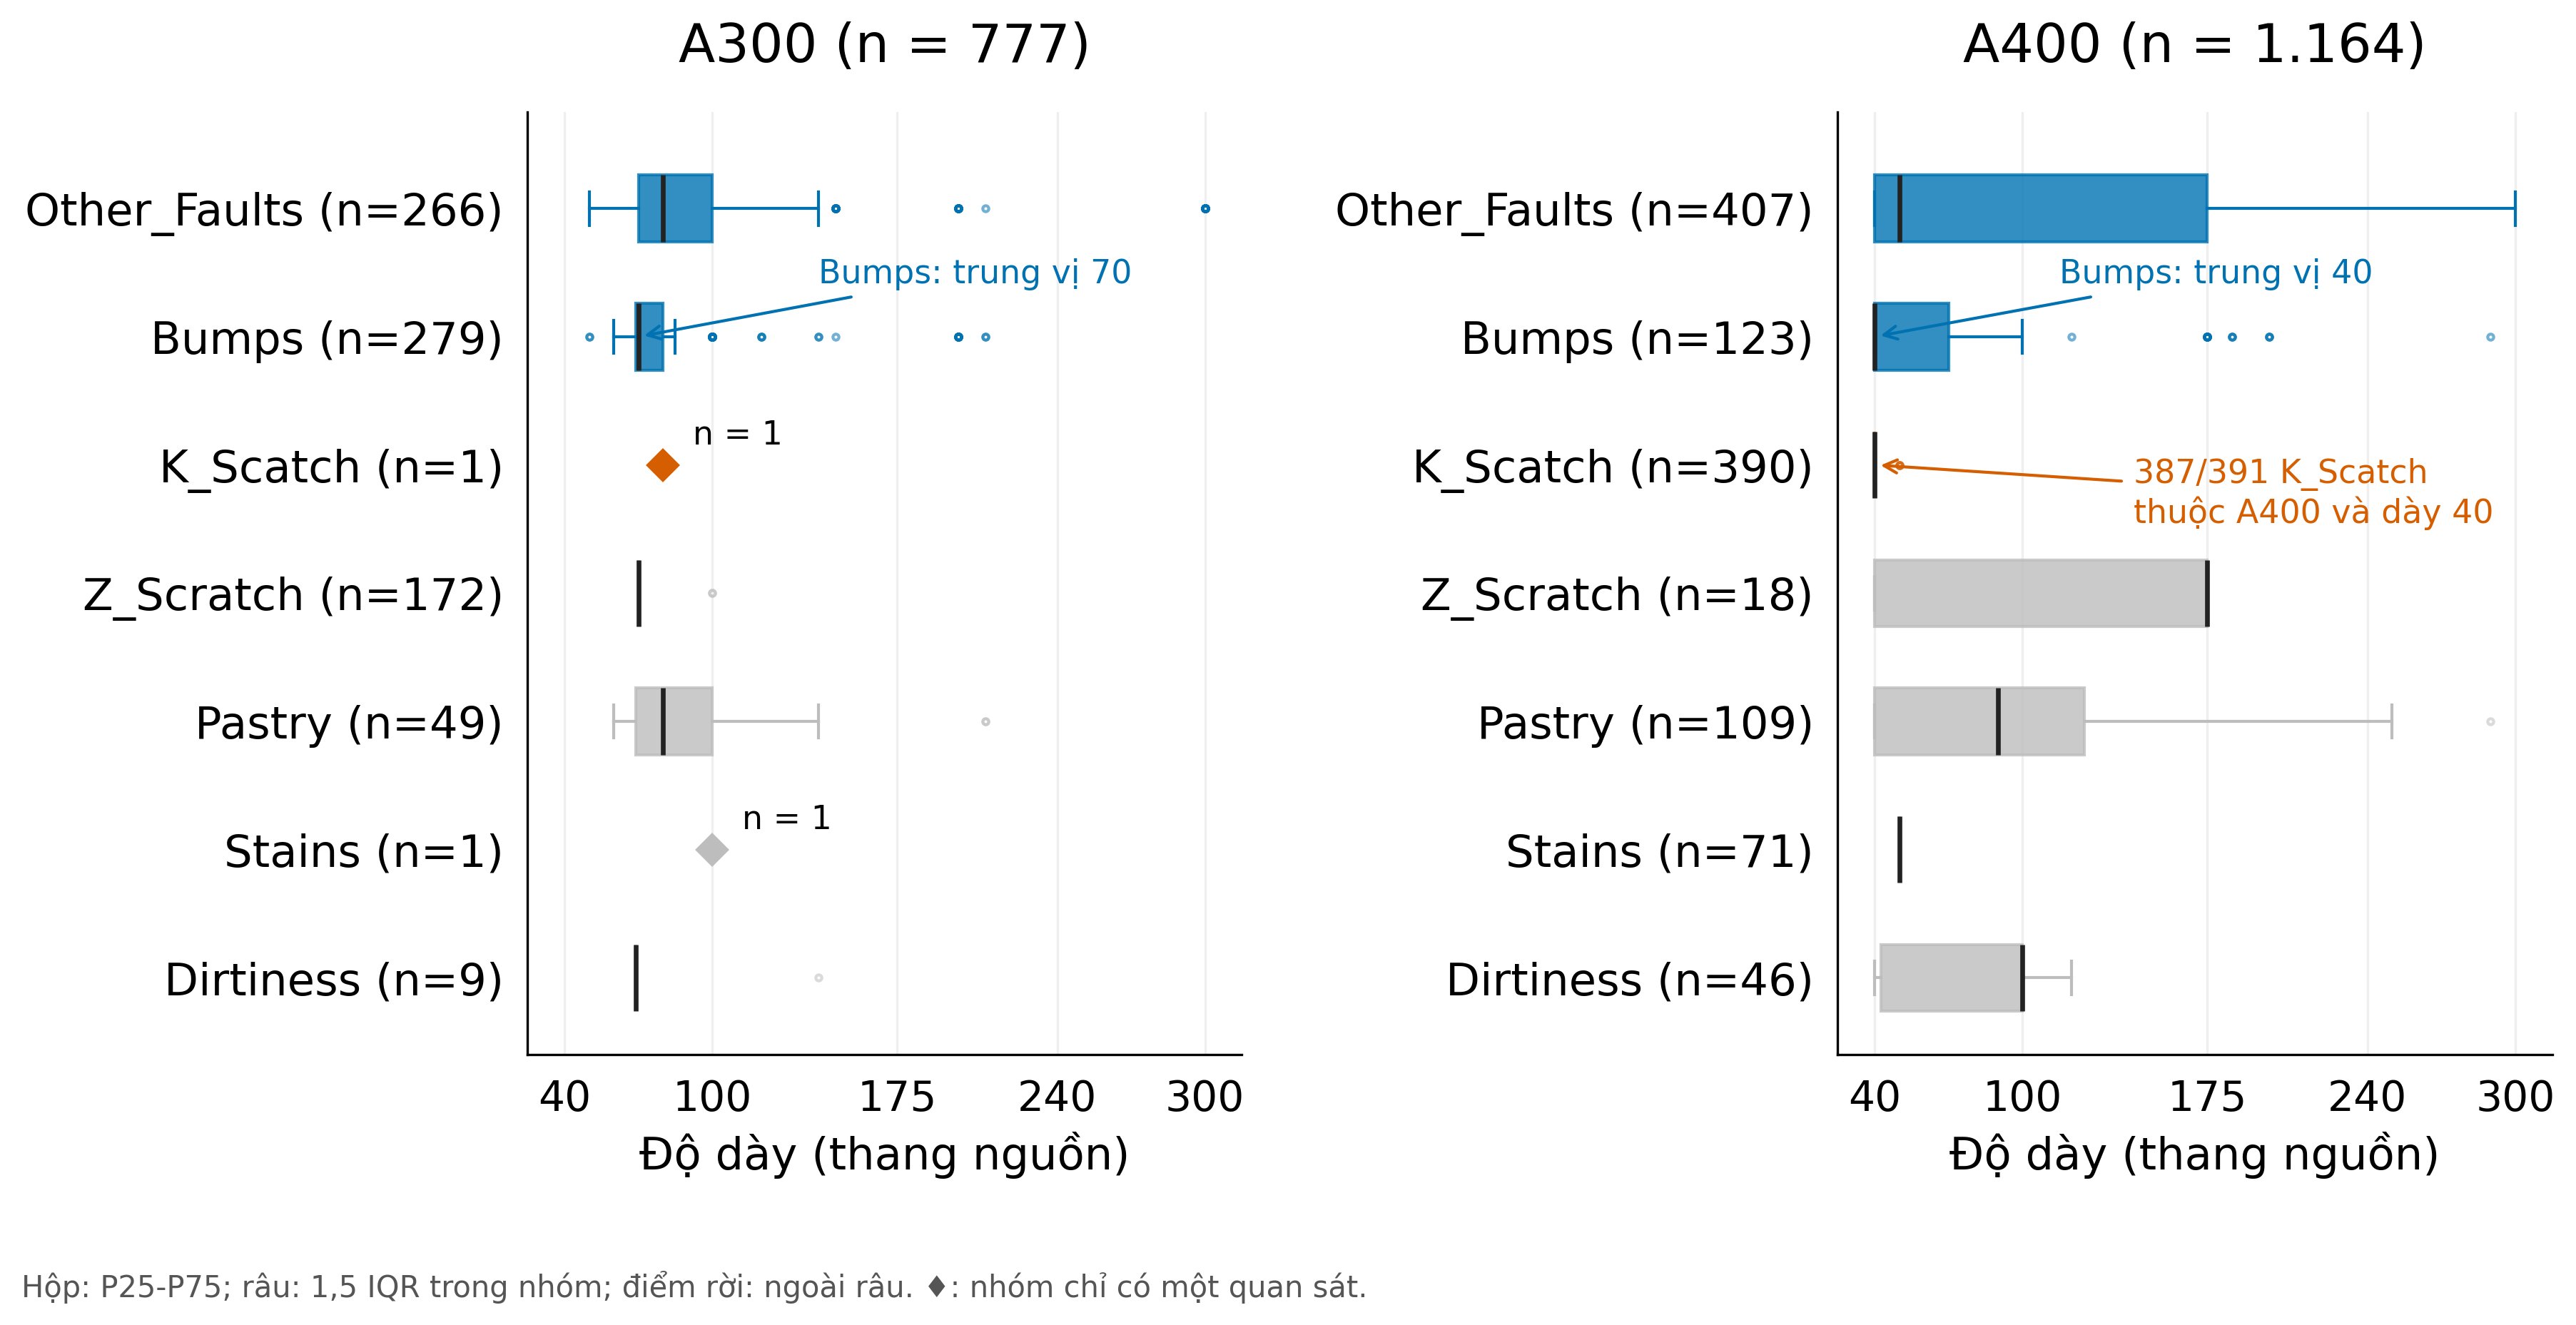
\includegraphics[width=\linewidth]{figures/chuong4/ch4_06_do_day_theo_thep.png}
\captionof{figure}{Cùng một nhãn, phân bố độ dày thay đổi theo dòng thép}
\label{fig:ch4dodaythep}
\end{minipage}\end{center}

\begin{center}\begin{minipage}{\linewidth}
\captionof{table}{Cỡ mẫu và trung vị độ dày trong từng tổ hợp nhãn--dòng thép}
\label{tab:ch4dodaythep}
\small\setstretch{1.1}
\begin{tabularx}{\linewidth}{@{}Y rrrr@{}}
\toprule
Nhãn & $N$ A300 & Trung vị A300 & $N$ A400 & Trung vị A400 \\
\midrule
\maCot{Other_Faults} & 266 & 80 & 407 & 50 \\
\maCot{Bumps} & 279 & 70 & 123 & 40 \\
\maCot{K_Scatch} & 1 & 80 & 390 & 40 \\
\maCot{Z_Scratch} & 172 & 70 & 18 & 175 \\
\maCot{Pastry} & 49 & 80 & 109 & 90 \\
\maCot{Stains} & 1 & 100 & 71 & 50 \\
\maCot{Dirtiness} & 9 & 69 & 46 & 100 \\
\bottomrule
\end{tabularx}
\end{minipage}\end{center}

Bảng cũng chứa những ô cần đọc thận trọng. \maCot{Z_Scratch} trên A400 có trung vị 175, nhưng chỉ dựa trên 18 bản ghi. \maCot{K_Scatch}/A300 và \maCot{Stains}/A300 mỗi tổ hợp chỉ có một quan sát, nên không mô tả được phân bố nào.

Nối Q2 với Q4, hồ sơ của \maCot{K_Scatch} trở nên rất hẹp: 387/391 bản ghi, tức 98,98\%, vừa thuộc A400 vừa có độ dày 40. \maCot{Stains} cũng tập trung ở A400 nhưng tại độ dày 50, với 71/72 bản ghi. Cùng một dòng thép vẫn có những nhóm mang hồ sơ khác nhau. Dữ liệu chưa cho phép tách vai trò riêng của dòng thép và độ dày, vì hai yếu tố này gần như trùng nhau trong nhóm \maCot{K_Scatch}.

\section{Diện tích, và cái giá của một ngưỡng chung: Q5}
\label{sec:ch4q5}

\subsection{Hai đầu của thang diện tích}

Ở Q1, \maCot{K_Scatch} và \maCot{Bumps} gần như ngang nhau về số lượng. Diện tích đặt chúng ở hai vị trí cách xa nhau: trung vị của \maCot{K_Scatch} là 6.281 pixel, của \maCot{Bumps} là 120,5 pixel. Ở đầu nhỏ nhất của thang là \maCot{Stains}, với trung vị 16,5 pixel, nhỏ hơn \maCot{K_Scatch} khoảng 381 lần. Trên Hình~\ref{fig:ch4boxarea}, khoảng P25--P75 của \maCot{K_Scatch} (3.948,5--10.908,5) nằm trên IQR của mọi nhãn khác, còn khoảng của \maCot{Stains} (13,5--18) nằm dưới tất cả. Các nhóm ở giữa chồng lên nhau nhiều.

\begin{center}\begin{minipage}{\linewidth}
\centering
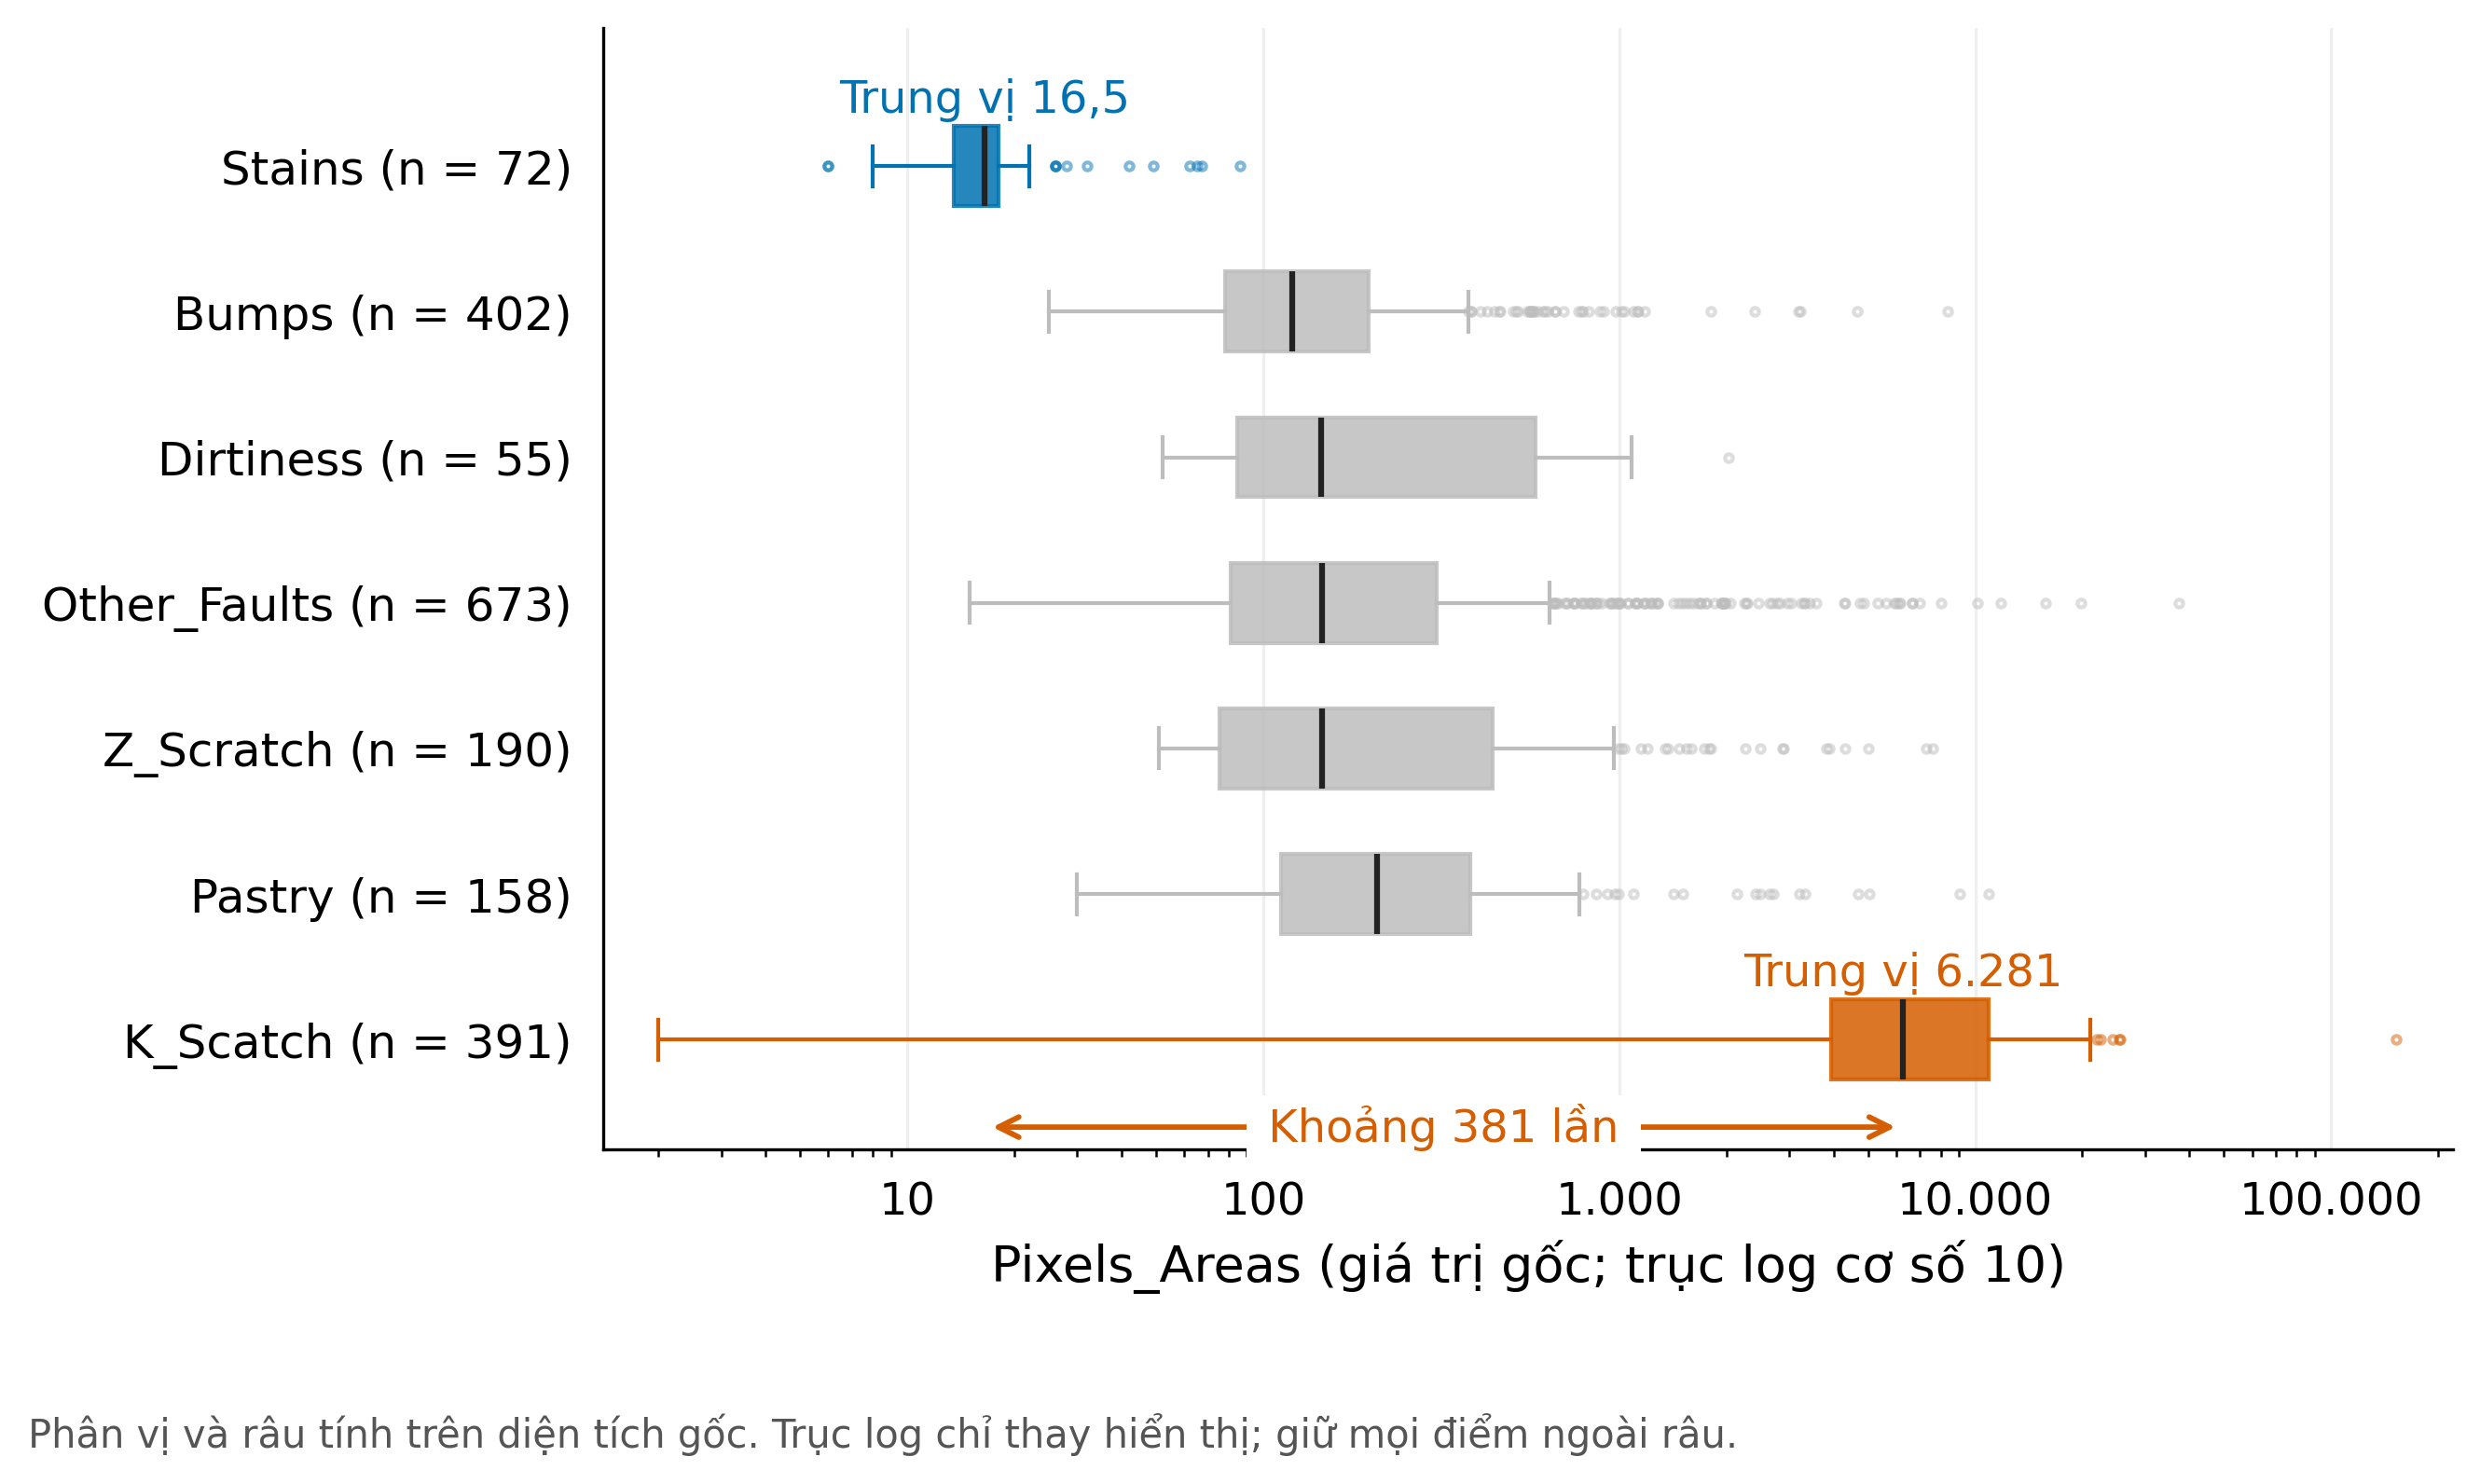
\includegraphics[width=\linewidth]{figures/chuong4/ch4_07_boxplot_dien_tich.png}
\captionof{figure}{K\_Scatch và Stains nằm ở hai đầu của thang diện tích}
\label{fig:ch4boxarea}
\end{minipage}\end{center}

\begin{center}\begin{minipage}{\linewidth}
\captionof{table}{Thống kê diện tích và số bản ghi ngoài râu theo từng nhãn}
\label{tab:ch4area}
\small\setstretch{1.1}
\begin{tabularx}{\linewidth}{@{}Y r p{3.1cm}r r r@{}}
\toprule
Nhãn & Trung vị & P25--P75 & Nhỏ nhất & Lớn nhất & Ngoài râu \\
\midrule
\maCot{Other_Faults} & 146 & 81--308 & 15 & 37.334 & 103 \\
\maCot{Bumps} & 120,5 & 78,25--197,5 & 25 & 8.391 & 44 \\
\maCot{K_Scatch} & 6.281 & 3.948,5--10.908,5 & 2 & 152.655 & 6 \\
\maCot{Z_Scratch} & 146 & 75,25--442 & 51 & 7.579 & 23 \\
\maCot{Pastry} & 209 & 112,5--381,25 & 30 & 10.914 & 19 \\
\maCot{Stains} & 16,5 & 13,5--18 & 6 & 86 & 13 \\
\maCot{Dirtiness} & 145 & 84,5--581,5 & 52 & 2.028 & 1 \\
\bottomrule
\end{tabularx}
\smallskip
\par\raggedright\footnotesize Ngoài râu: số bản ghi nằm ngoài khoảng từ P25 trừ 1,5 lần IQR đến P75 cộng 1,5 lần IQR, tính riêng cho từng nhãn trên thang diện tích gốc.
\end{minipage}\end{center}

Diện tích lớn là đặc điểm phổ biến của \maCot{K_Scatch}, nhưng không phải của mọi bản ghi: chính nhóm này chứa bản ghi nhỏ nhất toàn tập, 2 pixel, bên cạnh bản ghi lớn nhất, 152.655 pixel.

\subsection{Nếu xóa ``ngoại lai'', K\_Scatch gần như biến mất}

Đến đây, quyết định giữ lại 395 bản ghi ở Q0 mới thấy hết ý nghĩa. Quy tắc IQR tính trên toàn tập (P25 = 84, P75 = 822, hàng rào trên 1.929) gắn cờ 395 bản ghi có diện tích lớn. Trong đó, 326 bản ghi thuộc \maCot{K_Scatch}, tức 83,38\% của nhãn này. Nếu tính IQR riêng trong từng nhãn, \maCot{K_Scatch} chỉ có sáu bản ghi ngoài râu. Nói cách khác, phần lớn những gì quy tắc toàn tập coi là ``ngoại lai'' chính là diện tích bình thường của \maCot{K_Scatch}.

Hình~\ref{fig:ch4xoaco} và Bảng~\ref{tab:ch4xoaco} cho thấy hệ quả nếu xóa toàn bộ 395 bản ghi này. Tập dữ liệu còn 1.546 dòng, \maCot{K_Scatch} còn 65 bản ghi, tỷ trọng giảm từ 20,14\% xuống 4,20\% và thứ hạng tụt từ thứ ba xuống thứ sáu. Các nhãn khác gần như không bị ảnh hưởng: \maCot{Stains} giữ nguyên 72 bản ghi, \maCot{Bumps} chỉ mất 5.

\begin{center}\begin{minipage}{\linewidth}
\centering
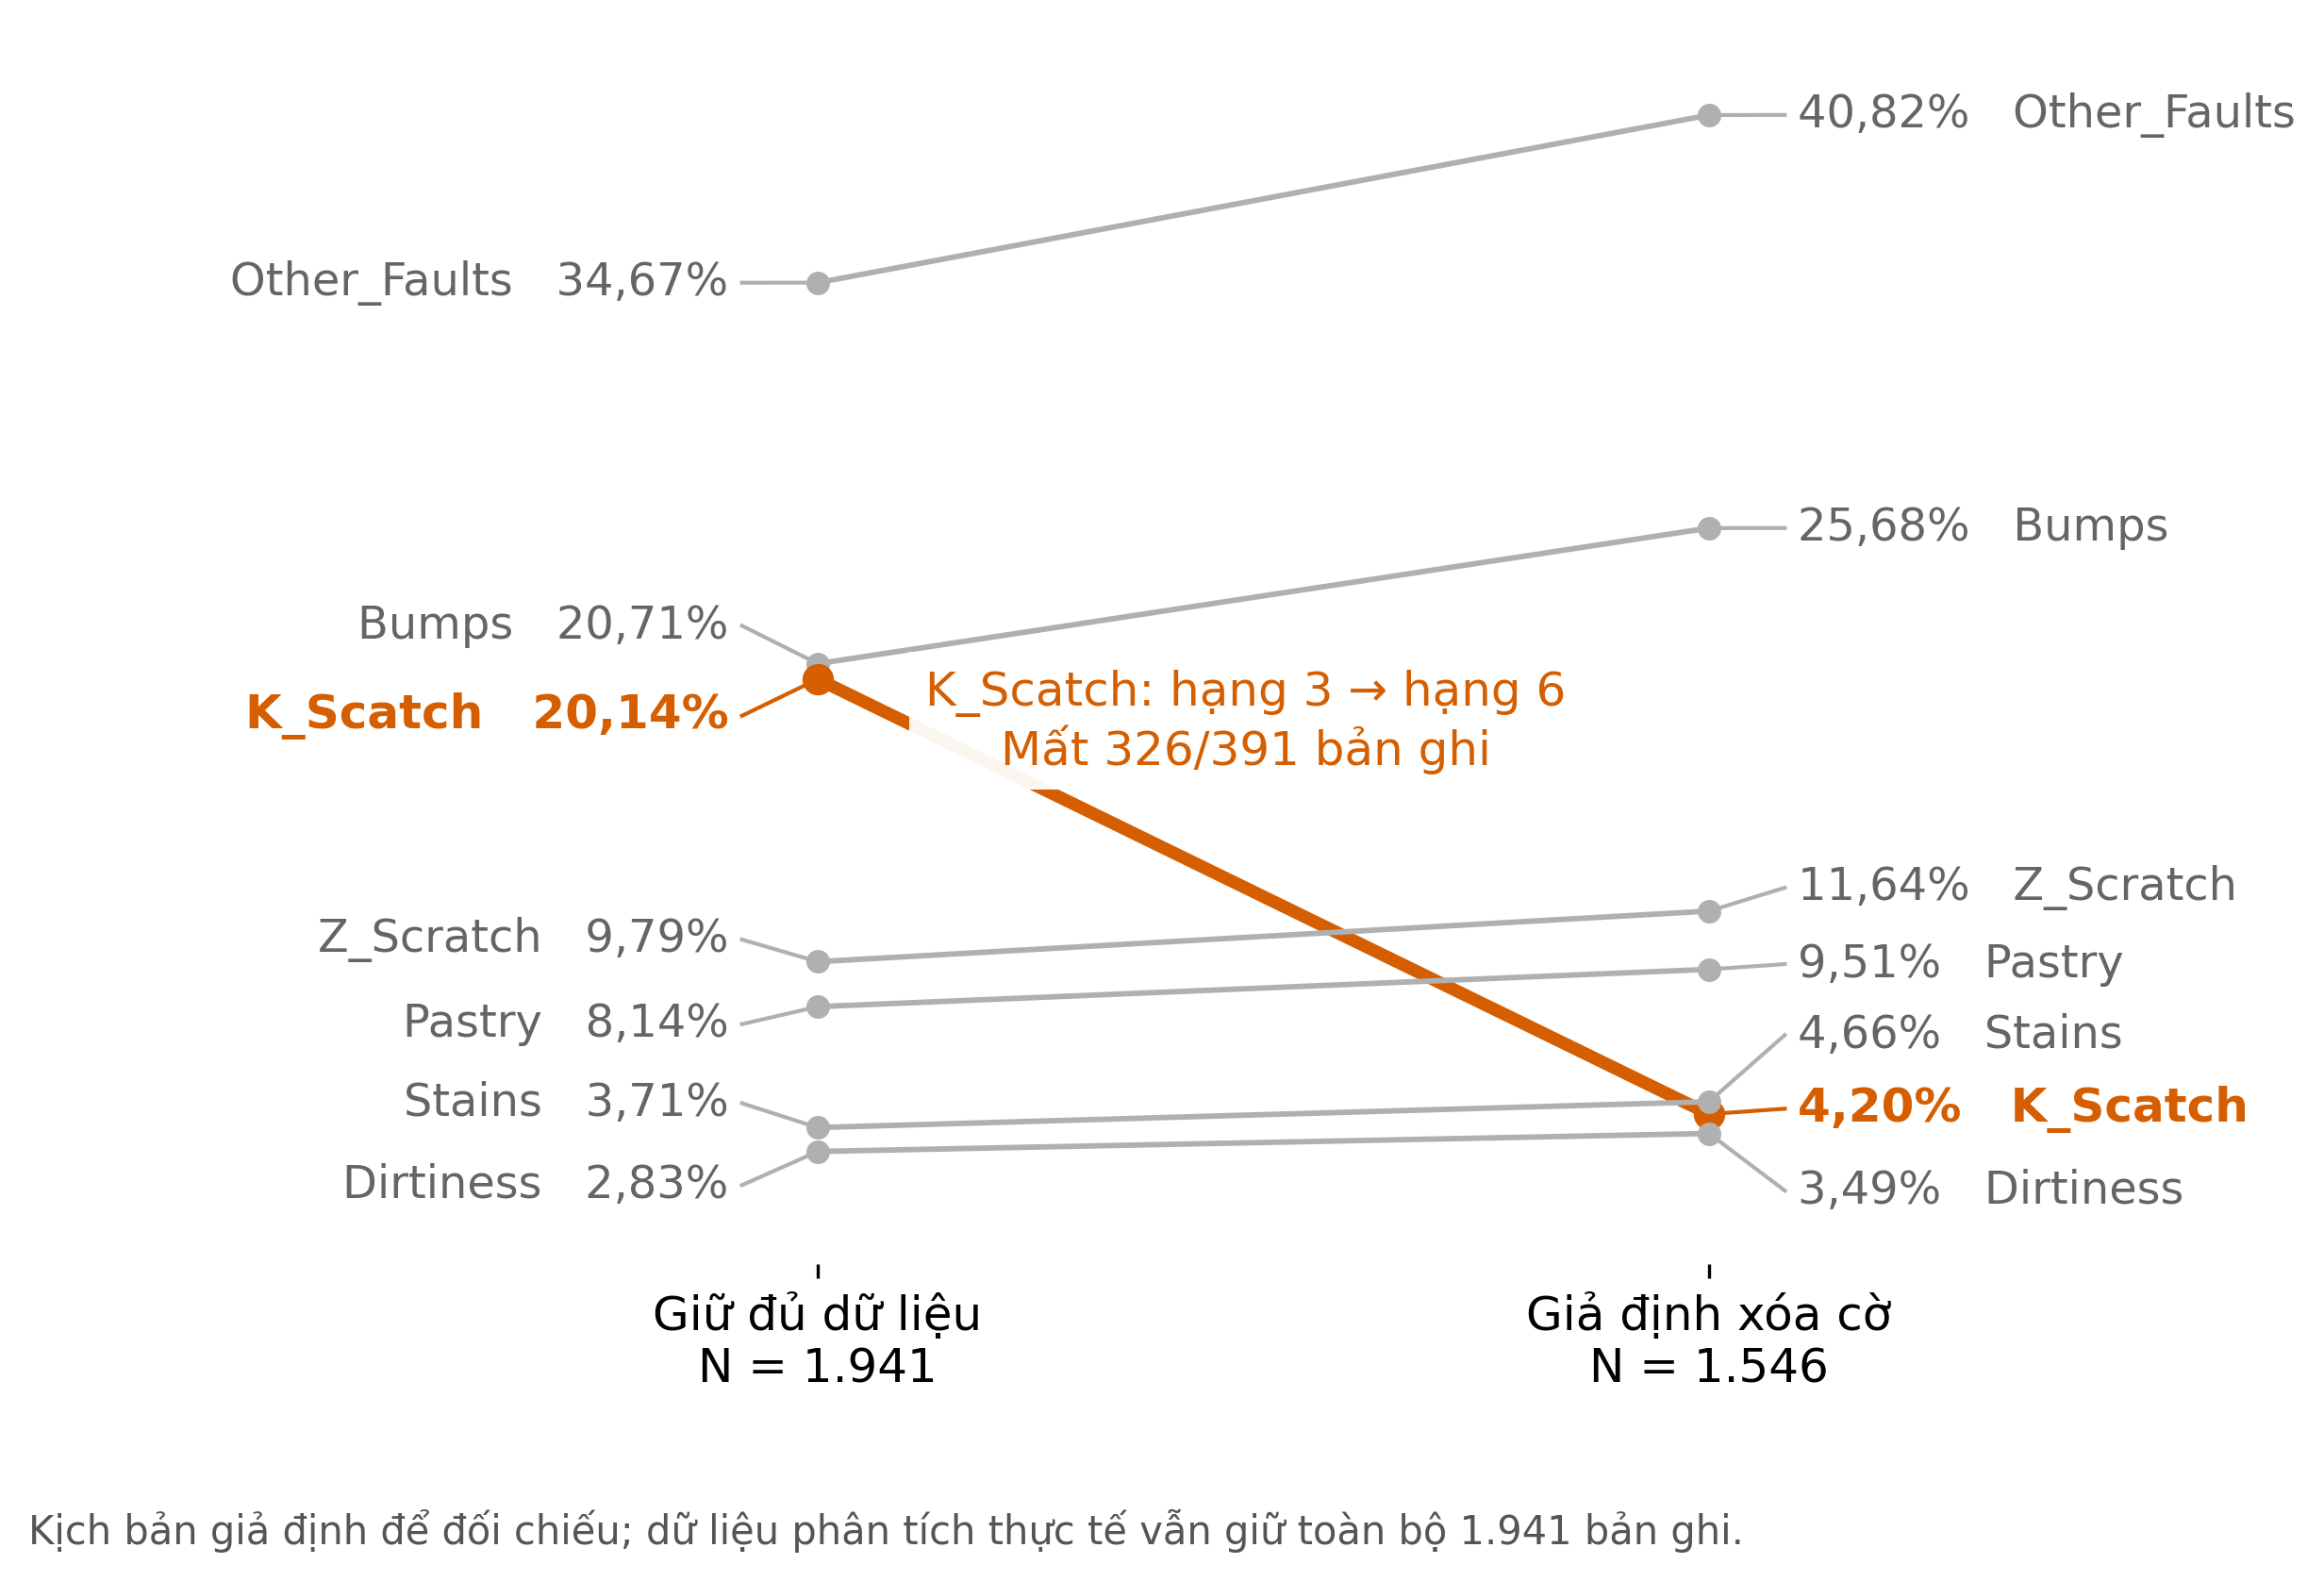
\includegraphics[width=\linewidth]{figures/chuong4/ch4_08_truoc_sau_xoa_co.png}
\captionof{figure}{Xóa cờ diện tích theo ngưỡng chung sẽ xóa gần hết K\_Scatch khỏi cơ cấu}
\label{fig:ch4xoaco}
\end{minipage}\end{center}

\begin{center}\begin{minipage}{\linewidth}
\captionof{table}{Cơ cấu nhãn khi giữ đủ dữ liệu và khi xóa 395 bản ghi bị gắn cờ diện tích}
\label{tab:ch4xoaco}
\small\setstretch{1.1}
\begin{tabularx}{\linewidth}{@{}Y rr r rr@{}}
\toprule
Nhãn & Giữ đủ & Tỷ trọng (\%) & Số cờ & Sau khi xóa & Tỷ trọng (\%) \\
\midrule
\maCot{Other_Faults} & 673 & 34,67 & 42 & 631 & 40,82 \\
\maCot{Bumps} & 402 & 20,71 & 5 & 397 & 25,68 \\
\maCot{K_Scatch} & 391 & 20,14 & \textbf{326} & \textbf{65} & \textbf{4,20} \\
\maCot{Z_Scratch} & 190 & 9,79 & 10 & 180 & 11,64 \\
\maCot{Pastry} & 158 & 8,14 & 11 & 147 & 9,51 \\
\maCot{Stains} & 72 & 3,71 & 0 & 72 & 4,66 \\
\maCot{Dirtiness} & 55 & 2,83 & 1 & 54 & 3,49 \\
\midrule
Tổng & 1.941 & 100,00 & 395 & 1.546 & 100,00 \\
\bottomrule
\end{tabularx}
\smallskip
\par\raggedright\footnotesize Kịch bản giả định để đối chiếu; dữ liệu phân tích thực tế giữ lại toàn bộ 1.941 bản ghi.
\end{minipage}\end{center}

Đây là điểm nút của chương. Một bước làm sạch tưởng như kỹ thuật, ``loại ngoại lai'', nếu làm tự động theo ngưỡng chung sẽ xóa đi gần trọn nhóm có hồ sơ rõ nhất trong dữ liệu, và biểu đồ cơ cấu sau đó sẽ kể một câu chuyện hoàn toàn khác. Việc giữ lại các bản ghi có căn cứ nguồn ở Q0 vì thế không chỉ là cẩn trọng về thủ tục; nó quyết định những gì các biểu đồ trong chương này có thể cho thấy.

Tổng hợp lại, \maCot{K_Scatch} là nhóm thứ ba về số lượng, nhưng gần như nằm trọn trên A400, ở độ dày 40, có phần trung tâm độ sáng tối thiểu thấp và diện tích lớn. Dashboard cho phép người đọc thu hẹp đúng vào nhóm này để kiểm tra lại hồ sơ đó.

\section{Kiểm tra lại câu chuyện trên dashboard}
\label{sec:ch4dashboard}

\subsection{Thu hẹp phạm vi vào nhóm K\_Scatch trên A400}

Trên dashboard, bộ lọc dòng thép, nhãn và khoảng độ dày xác định một tập con; KPI, biểu đồ và bảng đều tính trên tập con đó. Ở phạm vi toàn bộ (Hình~\ref{fig:ch4dashboardall}), giao diện hiển thị 1.941 bản ghi, bảy nhãn, trung vị diện tích 174,0 và trung vị độ dày 70,0.

\begin{center}\begin{minipage}{\linewidth}
\centering
\ghiChuHinh{Ảnh chụp dashboard thật đang chờ bổ sung: chọn A300 và A400, cả bảy nhãn, toàn khoảng độ dày. Cần hiển thị bộ lọc và KPI 1.941; 7; 174,0; 70,0. Tệp: \maCot{figures/chuong4/ch4_09_dashboard_toan_bo.png}.}
\captionof{figure}{Dashboard ở phạm vi toàn bộ dữ liệu lỗi}
\label{fig:ch4dashboardall}
\end{minipage}\end{center}

Khi chỉ chọn A400 và \maCot{K_Scatch} (Hình~\ref{fig:ch4dashboardfilter}), số bản ghi còn 390, trung vị diện tích tăng lên 6.281,5 và trung vị độ dày giảm xuống 40,0. Hồ sơ đã mô tả ở các mục trước hiện ra trực tiếp trên KPI. Trung vị 6.281,5 hơi khác giá trị 6.281 ở Q5 vì bộ lọc đã loại bản ghi \maCot{K_Scatch} duy nhất trên A300.

\begin{center}\begin{minipage}{\linewidth}
\centering
\ghiChuHinh{Ảnh chụp dashboard thật đang chờ bổ sung: chỉ chọn A400 và K\_Scatch, giữ toàn khoảng độ dày. Cần hiển thị bộ lọc và KPI 390; 1; 6.281,5; 40,0. Tệp: \maCot{figures/chuong4/ch4_10_dashboard_a400_kscatch.png}.}
\captionof{figure}{Dashboard sau khi thu hẹp vào A400 và K\_Scatch}
\label{fig:ch4dashboardfilter}
\end{minipage}\end{center}

Bảng~\ref{tab:ch4kpi} ghi lại KPI ở một số phạm vi tiêu biểu để đối chiếu với giao diện. Khi không chọn nhãn nào, tập con rỗng có số bản ghi bằng 0 và hai trung vị hiển thị dấu gạch thay vì số 0, vì không có giá trị nào để tính.

\begin{center}\begin{minipage}{\linewidth}
\captionof{table}{KPI đối chiếu tại các phạm vi lọc tiêu biểu}
\label{tab:ch4kpi}
\small\setstretch{1.1}
\begin{tabularx}{\linewidth}{@{}Y r r r r@{}}
\toprule
Phạm vi & Số bản ghi & Số nhãn & Trung vị diện tích & Trung vị độ dày \\
\midrule
Toàn bộ & 1.941 & 7 & 174,0 & 70,0 \\
A300 & 777 & 7 & 113,0 & 70,0 \\
A400 và \maCot{K_Scatch} & 390 & 1 & 6.281,5 & 40,0 \\
Không chọn nhãn & 0 & 0 & -- & -- \\
\bottomrule
\end{tabularx}
\end{minipage}\end{center}

Tab dữ liệu--chất lượng giữ một phạm vi khác: nó phản ánh toàn bộ nguồn, nên số liệu không đổi khi bộ lọc lỗi thu hẹp. Nhờ vậy, người dùng phân biệt được hai câu hỏi thường nằm cạnh nhau trên một dashboard: dữ liệu nguồn đã được xử lý ra sao, và tập bản ghi nào đang được phân tích.

\subsection{Kiểm thử phạm vi và cập nhật}

Một ảnh chụp có số liệu hợp lý chưa chứng minh bộ lọc và cơ chế cập nhật hoạt động đúng. Bộ kiểm thử gồm 11 ca được chạy lại trên một bản sao cô lập của dự án, với mã hiện tại và đầu vào tương ứng, để có thể thử nguồn bị thay đổi hoặc bị lỗi mà không động đến dữ liệu của bài. Cả 11 ca đều đạt (Bảng~\ref{tab:ch4test}).

\begin{center}\begin{minipage}{\linewidth}
\captionof{table}{Các nhóm chức năng và bằng chứng kiểm thử dashboard}
\label{tab:ch4test}
\small\setstretch{1.1}
\begin{tabularx}{\linewidth}{@{}p{3.0cm}Y p{0.9cm}@{}}
\toprule
Nhóm chức năng & Tình huống và kết quả kiểm chứng & Kết quả \\
\midrule
Khởi động, thành phần & Hiển thị ba tab, chín biểu đồ, hai nút tải CSV; toàn bộ có 1.941 bản ghi. & Đạt \\
Bộ lọc, đặt lại & A300 còn 777; A300 và \maCot{K_Scatch} còn một; độ dày đúng khoảng; đặt lại về 1.941. & Đạt \\
Phạm vi rỗng & Không chọn nhãn cho 0 dòng và trung vị là dấu gạch; năm thương mại thiếu có thông báo. & Đạt \\
Nạp nguồn, giữ bản hợp lệ & Nguồn thử giảm một bản ghi làm kết quả còn 1.940; nguồn thiếu cột bị từ chối, giữ bản hợp lệ. & Đạt \\
Làm mới, chu kỳ & Nút làm mới gọi bộ đọc một lần; giả lập qua 301 giây gọi một lần; tắt tự động không gọi. & Đạt \\
Lỗi API, nguồn bổ sung & Mất mạng giữ bản cũ; HTTP 429 thử lại một lần; sai quốc gia bị từ chối. & Đạt \\
Nhất quán tính toán & Bảng phân tích, cơ cấu, hai mẫu số và thống kê khớp notebook; boxplot log giữ phân vị thang gốc. & Đạt \\
\bottomrule
\end{tabularx}
\end{minipage}\end{center}

Với người đọc kết quả, hai hành vi quan trọng nhất là giữ đúng phạm vi và phản ánh đúng nguồn. Bộ lọc trả về số bản ghi như dự kiến; khi nguồn thử bớt một bản ghi, kết quả cập nhật còn 1.940; khi nguồn thiếu cột, ứng dụng từ chối cập nhật và giữ bản hợp lệ trước đó.

Phạm vi kiểm thử cũng có giới hạn. Lỗi API được mô phỏng; chu kỳ năm phút được kiểm tra bằng cách giả lập thời gian, chưa theo dõi ứng dụng chạy liên tục nhiều giờ; tệp CSV tải qua trình duyệt và việc bộ nhớ đệm API hết hạn sau 15 phút chưa có ca kiểm thử riêng. Kết quả 11/11 xác nhận những tình huống đã thử, không đo mức độ dễ sử dụng hay hiệu quả trong sản xuất.

\section{Thảo luận kết quả và giới hạn}
\label{sec:ch4thaoluan}

\subsection{Từ tần suất đến hồ sơ của từng nhóm}

Câu chuyện của chương có thể tóm trong một câu: thứ hạng theo số lượng không cho biết nhóm nào có hồ sơ rõ nhất. \maCot{Other_Faults} đông nhất nhưng là nhãn gộp, phân tán rộng cả về độ dày lẫn diện tích. \maCot{Bumps} và \maCot{K_Scatch} gần như ngang nhau về số đếm, nhưng \maCot{K_Scatch} gần như nằm trọn trên A400, ở độ dày 40, có phần trung tâm độ sáng tối thiểu thấp và diện tích lớn. Mô tả này cụ thể hơn nhiều so với việc gọi \maCot{K_Scatch} là ``lỗi phổ biến thứ ba'', và chỉ ra đúng tổ hợp cần kiểm chứng tiếp.

\maCot{Stains} là một hồ sơ hẹp khác: ít bản ghi, tập trung ở A400, độ dày 50 và diện tích rất nhỏ. Tuy vậy, số đếm thấp hay diện tích nhỏ không nói gì về mức độ quan trọng của một loại lỗi; điều đó phụ thuộc vào tiêu chí chấp nhận, vị trí lỗi và thiệt hại thực tế, những thông tin không có trong dữ liệu. Với \maCot{Other_Faults}, bước hợp lý tiếp theo là xem lại định nghĩa nhãn và ảnh bề mặt trước khi nghĩ đến việc chia nhỏ.

Mục~\ref{sec:ch4q5} còn cho thấy một bài học về quy trình: cách xử lý giá trị ngoại lai có thể quyết định nội dung của biểu đồ. Nếu \maCot{K_Scatch} bị xóa gần hết bởi một ngưỡng chung, toàn bộ hồ sơ vừa mô tả sẽ không xuất hiện.

\subsection{Đặt từng kết luận trong phạm vi bằng chứng}

Bảng~\ref{tab:ch4bangchung} phân biệt ba loại nội dung: kết quả tái tính được từ dữ liệu, nhận định cần kiểm tra thêm, và kết luận còn thiếu căn cứ.

\begin{center}\begin{minipage}{\linewidth}
\captionof{table}{Phân biệt kết quả mô tả, nội dung cần kiểm tra và kết luận chưa đủ căn cứ}
\label{tab:ch4bangchung}
\small\setstretch{1.1}
\begin{tabularx}{\linewidth}{@{}p{0.8cm}Y Y@{}}
\toprule
Mức & Nội dung & Căn cứ hoặc phần còn thiếu \\
\midrule
A & Cơ cấu nhãn, tỷ trọng A300/A400, trung vị, IQR, số điểm ngoài râu, kịch bản xóa cờ; các ca chức năng đã đạt. & Tái tính được từ bảng và kiểm thử; có hiệu lực trong dữ liệu, phạm vi đã nêu. \\
B & Độ sáng thấp có thể hỗ trợ nhận diện \maCot{K_Scatch}; cần xem kỹ tổ hợp A400--độ dày 40. & Cần dữ liệu độc lập, đủ quan sát trong từng tổ hợp và đánh giá sai nhãn. \\
C & Dòng thép dễ lỗi hơn, nguyên nhân vật lý, nhãn gây thiệt hại lớn nhất hoặc xu hướng sản xuất theo thời gian. & Thiếu sản lượng, điều kiện vận hành, chi phí, định danh sản phẩm và thời gian thực. \\
\bottomrule
\end{tabularx}
\smallskip
\par\raggedright\footnotesize A/B/C là quy ước trình bày của bài để phân biệt phạm vi bằng chứng, không phải thang điểm hay mức tin cậy thống kê.
\end{minipage}\end{center}

Các giới hạn sau áp dụng cho toàn bộ câu chuyện ở trên.

\emph{Về mẫu số.} Tập dữ liệu chỉ gồm bản ghi lỗi, không có tổng sản lượng đạt và không đạt. Mọi tỷ trọng ở Q1--Q2 mô tả cơ cấu trong tập lỗi; chúng chưa cho biết xác suất phát sinh lỗi của một dòng thép. Thiếu định danh tấm hoặc cuộn cũng khiến tính độc lập giữa các bản ghi chưa được xác nhận.

\emph{Về xử lý dữ liệu.} Khôi phục theo UCI giúp tái lập bảng tham chiếu, nhưng độ đúng của giá trị sau khôi phục phụ thuộc vào chính nguồn đó và vào việc ghép đúng bản ghi. Kết quả phát hiện 16 ô bằng quan hệ nội tại chỉ có hiệu lực với những trường đã đặt quy tắc, và các quy tắc này được rà soát sau khi đã biết vị trí lỗi.

\emph{Về cách đọc biểu đồ.} Scatter có nhiều điểm chồng lấn; IQR chỉ mô tả phần trung tâm; nhóm $N=1$ không cho biết độ phân tán. Tiêu chí không chồng IQR ở Q3 được đặt ra sau khi quan sát dữ liệu, nên dấu hiệu độ sáng cần được kiểm tra trên dữ liệu khác trước khi dùng để nhận diện nhãn. Ở \maCot{K_Scatch}, dòng thép và độ dày gần như trùng nhau, nên chưa tách được vai trò riêng của từng yếu tố.

\emph{Về phạm vi dữ liệu.} Ngày đã chuẩn hóa là ngày mô phỏng, không hỗ trợ kết luận về diễn biến theo thời gian. Nguồn thương mại ở phụ lục không có khóa liên hệ với bản ghi lỗi và không được dùng để giải thích Q1--Q5. Dashboard có bằng chứng chức năng trong các tình huống đã thử; đánh giá với người dùng tại nhà máy vẫn là công việc tiếp theo.

\section{Tiểu kết chương và hướng hoàn thiện}

Chương bắt đầu từ một bảng dữ liệu có thể kiểm tra lại và kết thúc bằng một hồ sơ cụ thể. Q0 xác lập cơ sở để tin các biểu đồ; Q1 cho thấy số lượng tập trung ở ba nhãn; Q2--Q5 lần lượt làm hiện ra \maCot{K_Scatch} như nhóm có hồ sơ rõ nhất: A400, độ dày 40, độ sáng tối thiểu thấp ở phần trung tâm và diện tích lớn. Kịch bản xóa cờ ở Q5 cho thấy hồ sơ này chỉ hiện ra được vì các quan sát có căn cứ nguồn đã được giữ lại. Dashboard cho phép người đọc thu hẹp vào đúng nhóm này để kiểm tra, với 11 ca kiểm thử chức năng đạt trên phiên bản hiện tại.

Hướng tiếp theo đi thẳng từ những gì dữ liệu còn thiếu. Về dữ liệu, cần bổ sung sản lượng theo dòng thép và độ dày, định danh sản phẩm, thời gian sản xuất thực và mức độ thiệt hại. Về phân tích, cần kiểm tra lại dấu hiệu độ sáng của \maCot{K_Scatch} trên dữ liệu độc lập và làm rõ nhãn nghiệp vụ của \maCot{Other_Faults}. Về dashboard, cần kiểm thử tệp tải xuống, theo dõi cập nhật dài hạn và đánh giá với nhiệm vụ sử dụng thực tế.
